\section*{Project Description}

Testing plays a vital role in the robustness, security, and overall
quality of modern software. It comes in many styles---unit testing,
integration testing, performance testing, stress testing,
accessibility testing, penetration testing, etc.---supported by
diverse tools, with yet more advanced tools and methodologies always on
the horizon.

One such methodology is {\em property-based testing} (PBT),
sometimes described as ``formal specification without formal
verification.''  With PBT, a developer characterizes the desired
behavior of
some piece of code in the form of executable {\em
  properties}. The code is
then validated against these properties by running it many times
with a large number of automatically generated test
inputs.
%
% PBT thus achieves a comprehensiveness that is often not
% possible with alternative testing methods. \iflater\bcp{Why not with
%   fuzzing??  Can we say it explicitly, to avoid leaving a question
%   pending for some readers?}\fi
%
This combination of rich, high-level specifications and mostly
automatic validation has proven effective at identifying
subtle bugs in a wide variety of settings, including
telecommunications software~\cite{arts2006testing}, replicated
file and key-value
stores~\cite{MysteriesOfDropbox2016,Bornholt2021}, automotive
software~\cite{arts2015testing}, and other complex
systems~\cite{hughes2016experiences}.
It is used by companies including Amazon, Volvo, Stripe, Galois,
and IOG, which
runs the Cardano blockchain and the Ada cryptocurrency.

PBT took the functional programming world by storm following its
debut in the Haskell QuickCheck framework~\cite{ClaessenHughes00}.  In
2010 the
QuickCheck authors received the ACM SIGPLAN ``Most Influential Paper of ICFP
2000'' for their paper on it; this is currently the most cited
ICFP paper by
a factor of 2, according to ACM's digital library.  In the intervening
years, PBT has spread to many other software ecosystems:
%
Wikipedia lists QuickCheck variants in 40  languages, some
with several competing frameworks~\cite{QuickCheckWikipedia} (Java alone has
7!).
%
And these frameworks are popular:
the developers of the Python Hypothesis framework~\cite{maciver2019hypothesis,HypothesisGithub} estimate its user community
at half a million~\cite{ZacPersonalCommunication,noauthor_python_nodate}.  On GitHub,
Hypothesis has 6.5K ``stars'' from developers (indicating enthusiasm)~\cite{borges_whats_2018}, Rust's
quickcheck~\cite{RustQuickcheckGithub} has 2K,
ScalaCheck~\cite{ScalaCheckGithub} has 1.8K, and Clojure's
test.check~\cite{ClojureTest.checkGithub} has 1.1K.
By comparison, pytest, the main framework Python users use to run
tests, has 9.6K stars~\cite{PytestGitHub}---i.e., Python's
PBT tool has around 70\% as many stars as Python's entire testing
infrastructure.

And there is still plenty of room
for growth.
The 500K estimate for
Hypothesis users is only 4\% of all Python developers; the Hypothesis
authors estimate that the ``addressable market'' for PBT is around
25\% of the Python
community, and that there remains significant room for
improving its usage by existing users~\cite{ZacPersonalCommunication,noauthor_python_nodate}.
Similarly, the list of
companies using PBT, while substantial, is very far from the whole of the software
industry.
These gaps represent a gigantic opportunity to increase software quality
and reduce software costs.
A 2002 study~\cite{2002economic} estimated that the total cost of software errors is almost
\$60 billion per year and suggested that \$22 billion of that could be
saved through
better testing infrastructure; since then, the situation has only gotten worse, with a 2022
study~\cite{krasner2022cost} estimating that poor software quality now
costs the U.S.{} over \$2 trillion per
year. Accelerating the adoption of PBT thus stands to make a
significant dent
in the global cost of software bugs.  This is the grand challenge that
we address.

Our group has already begun working to identify
high-leverage ways to extend PBT's reach.
In an ongoing need-finding study with PBT users at Jane Street
Capital, we found consistent enthusiasm---developers called it
``obviously valuable'' (Participant \participant{1}), built their own
frameworks for it when standard ones were not available
(\participant{8}, \participant{21}), and suggested that ``everyone''
at the company should use it (\participant{20}); however, developers
also highlighted a key opportunity for improvement---{\em usability}.
%
Like
many powerful tools, PBT can be difficult to apply, and developers
need support to do so effectively.

% \amh{This is a deficit-focused pitch---focusing on the problems that need to be
% solved with PBT---rather than an asset-focused pitch---focusing on how we need
% new paradigms for PBT. Can we shift the focus of this to stating one big way in
% which innovation in PBT is necessary?}
% Given all this momentum, one might wonder whether the research community
% has already discovered and addressed all of the challenges that might limit PBT's adoption
% in the broader software industry.  Sadly, it has not:
% in an ongoing need-finding study with users of OCaml's QuickCheck testing tool
% at Jane Street Capital, we have found
% consistent enthusiasm for PBT---participants called it
% ``obviously valuable'' (Participant \participant{1}),
% built their own libraries for it when standard ones were not available
% (\participant{8},
% \participant{21}), and suggested that ``everyone'' at the company should use it
% (\participant{20})---but participants also described {\em usability} issues that
% limit PBT's impact on the broader software community.

% Solving these issues
% requires advances in both technical foundations and
% tool design.\iflater\bcp{The last part of that sentence kind of
%   duplicates the first part of the next...}\fi

The research advances required to improve the usability of PBT
will require fundamental insights from
both the
programming languages (PL) and human-computer interaction (HCI),
communities.
On one side, PL provides conceptual background,
mathematical underpinnings, and established tools for PBT.  On the
other, HCI provides a deep foundation of theory and
practice for evaluating usability of systems in a
rigorous and objective way, including principled methods for
identifying problems, rigorous metrics, and proven
approaches to tool design---where tools, here, naturally include
``front end'' components like
data visualizers and IDE plug-ins, but
also ``back end'' technologies like domain-specific languages for
properties and generators; for the latter, HCI techniques
can help designers
strike the right balance between expressiveness and
accessibility~\cite{coblenz_pliers_2021,greenman_little_2022}.
Synergies like these led
Chasins et al.~\cite{chasins_pl_2021} to argue that a research
methodology combining PL and HCI hits a ``sweet spot'' where
need-finding techniques identify current
pain points, motivating concrete tools that help programmers write
safe, correct code.

% We intend to employ those particularly in the front-end aspect (the IDE for PBT);
% \item But also in the back-end (to strike the right balance between expressiveness and accessibility in our languages and libraries).
% \item For justification of the back-end language stuff, see the PLIERS paper
% % https://dl-acm-org.proxy.library.upenn.edu/doi/abs/10.1145/3452379
%  which provides a recipe for user-centered language design, and Little Tricky Logic
% % https://users.cs.utah.edu/~blg/resources/talks/vardifest-2022.pdf
% which argues that languages PL people like are often very confusing, and HCI methods can prevent us from designing languages that users won’t understand.
% \end{itemize}
% To provide tools for evaluating what we build that are faster and more direct than just putting things out into the world and waiting to see if users adopt them.

% Success in all these efforts will require complementary tools from PL and
% HCI research. HCI approaches will be used to concretely define
% developers' needs, design the user interface to tools, and evaluate
% their success, while PL techniques will be used to develop powerful
% domain-specific languages and type-based automation to improve the PBT
% process\proposecut{, as well as to formally validate these tools}.

Our team
is uniquely positioned to bring PBT into this vibrant area
of ``PL+HCI'' research.  PI Head recently
co-founded a new HCI group at
the University of Pennsylvania and specializes in interactive
programming environments, while PI Pierce has published widely on PL
topics including PBT.  Our past research collaboration has led to
two workshop
presentations~\cite{goldstein_problems_2022,shi_towards_2023} and to the ongoing
study at Jane Street mentioned above, which informs the
research and technology transfer agenda for the present proposal.

\smallskip

We propose an interdisciplinary program of research and
engineering in
{property-based testing}, bringing to
bear the combined power of PL and HCI to accelerate PBT's transition
into practice.
%
Planned research,
engineering, and education activities can be grouped into five main
themes (see Figure~\ref{overview}):
%
\begin{enumerate}[noitemsep]
% \begin{itemize}[noitemsep]
% \begin{enumerate*}
\item We will establish a solid \thread{foundation} for HCI-informed research on PBT,
building on our ongoing need-finding study. We will confirm and generalize
this study's findings through further studies, culminating in a novel
cognitive theory of PBT (\sectionref{sec:foundation}).
%
\item We will explore and apply a novel ``reflective'' approach to
\thread{generation}, enabling better generator tuning and counterexample
shrinking and linking PBT with fuzzing.  We will automate construction
of reflective generators, and we will construct a platform for
benchmarking these and other advances in tools for generation (\sectionref{sec:gen}).

% \item We will help developers efficiently define and tune random input
% \thread{generators} with novel techniques for generating values
% satisfying given preconditions, for test input mutation, and for
% example-based generator tuning---all building on a novel
% ``reflective'' approach to generation (\sectionref{sec:gen}).
%
\item We will empower developers to \thread{specify} properties with new
languages for expressing properties, tools that simplify the process of authoring
properties, and assistants that help to explain properties to others
(\sectionref{sec:spec}).
% tools for checking temporal properties over internal program states
% and for model-based testing of modularized code\proposecut{ and for authoring
% properties}, plus a comprehensive review of PBT practice to help
% students and developers identify situations where PBT is likely to be
% most useful\bcplater{the latter belongs under diffusion now, I
%   believe}
%
\item We will design, prototype, and evaluate novel tools for
\thread{interacting} with properties
and generators, leveraging our advances in specification and generation to
enable new ways of visualizing and understanding random distributions
over test inputs and pinpointing the cause of test failures.
(\sectionref{sec:val}).
%
\item We will support the \thread{diffusion} of PBT tools and
methodologies from academia into industry through targeted
engineering---in particular, supporting and
improving open-source PBT frameworks and building a comprehensive IDE
for PBT, dubbed \tyche.
We will also drive diffusion via education, developing materials for teaching
software developers about high-value applications of PBT and
for introducing PBT into undergraduate and masters-level computer science courses
(\sectionref{sec:diffusion}).
% \amh{Our diffusion efforts will also amplify
% future research efforts through the creation and dissemination of reference
% implementations for others to build on, and an extensible development
% environment that future HCI researchers can extend with new PBT affordances.}
% \end{enumerate*}
% \end{itemize}
\end{enumerate}
%
\begin{wrapfigure}{r}{.63\textwidth}
  \centering
  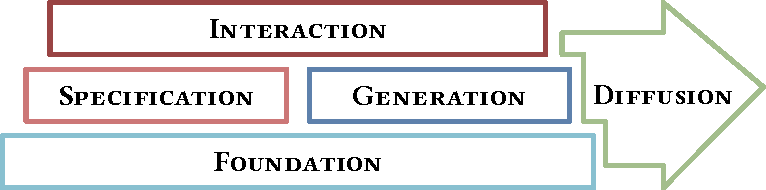
\includegraphics[width=.6\textwidth]{assets/overview.pdf}
  \caption{Overview of the proposed research. Four PhD students
  will advance the state of the art on four interconnected axes, supported by a
  research engineer and the PIs for maximum impact.}
  \label{overview}
\end{wrapfigure}
%
The scale of this project---two PIs, four PhD students, and a staff
engineer---is essential to the success of (1) its
tightly integrated research agenda, which requires expertise across PL and
HCI to make significant advances in the five interconnected themes above, and (2) its
goal of broad impact on industrial
practice, requiring the full-time attention of a software engineer.
%
A detailed sketch of responsibilities and timeline can be found in the
Management and Coordination supplement, but, briefly,
one PhD student will build on our existing user studies to
develop a clear foundational understanding of
PBT from the perspective of usability and human factors, two students
will develop ``back end'' technologies to support usable
PBT workflows, and a final student will leverage these technological
advances to design and develop ``front end'' IDE support. The
research engineer will focus on transferring the
products of this research into an industrial context, supporting and enriching
existing open-source PBT projects with theoretically informed ideas
and tools. None of these
projects stands on its own; rather, each supports and informs the
others to achieve both conceptual advances and significant
impact on software development practice.
%
Publication targets and other success metrics are discussed in each
section below.

Two PIs is on the small side for a Large NSF proposal, but  we feel this
is the right size, for two reasons. First, the PIs
come from quite distinct areas, so we already span a
broad swath of CS in terms of perspective and expertise.  Second,
our success will depend on a high degree of
interaction and cross-fertilization between PL and HCI; this is much
easier with fewer PIs.

Our plans for Broadening Participation in Computing, described in a
supplemental document, are focused in two areas: (1) expanding an
existing NSF-REU program that brings undergraduates from
underrepresented groups to Penn for summer research experiences in
programming languages, and (2) increasing diversity in the TA roster
for Penn's introductory computer science course, which PI Pierce
co-teaches.

\medskip

The rest of this Project Description describes this research and
technology transfer agenda in detail.  Sections
\sectionref{sec:orientation} and \sectionref{sec:motivation} supply
background on PBT and present preliminary findings from our
ongoing study at Jane Street.
%
Sections \sectionref{sec:foundation} through
\sectionref{sec:diffusion} outline plans for each of the
themes listed above.
Section \sectionref{sec:broader-impacts}
discusses the Broader Impacts of the project, and
Section \sectionref{sec:prior} summarizes our prior
NSF-supported work.

\SIMPLESECTION{Orientation: Property-Based Testing}{sec:orientation}

% We begin in this section with some background on PBT and preliminary
% results from our ongoing study at Jane Street

% \subsectionstar{Property-Based Testing}
% \subsectionstar{Orientation: Property-Based Testing}
%
PBT%
% , famously popularized by Haskell's QuickCheck library
~\cite{hughes2007quickcheck}
is software testing method where
executable functions are used as partial
specifications of a component under test. For example, a developer might
write the following property for an \lstinline{insert}
function on binary search trees, taking an arbitrary tree \texttt{t}
and an integer
\texttt{x} as parameters:
\begin{lstlisting}
  prop_insert_correct x t  =  (is_bst t ==> is_bst (insert x t))
\end{lstlisting}
That is, if the original tree
is a BST, then it should remain
a BST after the insertion of \texttt{x},
where \lstinline{is_bst} is a function that checks whether a binary
tree is arranged so that each node's label is greater
than any label in its left subtree and less than any in its right
subtree.
% \rjmhlater{The example property you give looks like a type check:
% given a BST as
% input, insert returns a BST as result. The reader may easily think
% such a property is of interest only in dynamically typed
% languages... and that it is a rather trivial property even there. Of
% course, I understand that it really tests that the BST invariant is
% preserved by insert, a deep semantic property, but you are just
% assuming that the reader will remember that binary search trees need
% to satisfy an invariant, and will guess that is_bst checks that
% invariant. Be more explicit to avoid a risk of misunderstanding. }%
In general, such a property is a function that
accepts a generated
test input
and evaluates to \lstinline{True} if the test passes and
\lstinline{False} otherwise.
% This one, ``\verb|prop_insert_correct|'',
% checks that an insert operation on a binary search tree preserves the
% binary ordering of the tree.
Given a property, the PBT tool generates a
large number of inputs and
checks that the property yields \lstinline{True} for each one; any input
that causes the property to fail is reported to the user as a
{counterexample}.
%
Designing these properties is an example of
the {\em oracle problem}~\cite{barr_oracle_2015}, which arises in any kind of
automated testing where the user needs to define what it means for a program to
be correct.

Our research agenda focuses mostly on {\em random}
generation~\cite{hamlet1994random}, the dominant approach in PBT,
though many of our tools would also be applicable to alternatives
like enumerative test-case
generation~\cite{DBLP:conf/haskell/RuncimanNL08, leancheck}.  The
surprising effectiveness of random generation can be attributed to the
``combinatorial nature'' of large test cases---the fact that bugs can
often be exposed by any test input that embodies some specific combination
of features, independent of whatever other features may also be
present.  For example, a bug might be triggered by a particular
sequence of API calls in a particular order, even when
these are interleaved with other API calls. As a result, testing with
large random inputs often exposes issues much faster than exhaustively
enumerating small inputs.  Techniques like swarm
testing~\cite{groce2012swarm} can further amplify this effect.

To apply PBT to a system or an individual software component, the
developer first defines one
or more properties that they expect should always be satisfied. Then
they supply {\em random input generators} for the values that the
properties take as input---these are sometimes written by hand, but
often they can be automatically generated, e.g., from the type of the
input. Next, they check their properties against many generated
inputs, using a test harness provided by their PBT tool. And finally, if
counterexamples are discovered, they inspect them to determine the
source of the bug.  Each of these steps can be significantly improved for users,
as we describe in the next section.

\smallskip

Why go to the trouble of PBT, rather than the more straightforward
example-based testing that is standard across the software industry?
First and foremost because a component can be tested much more
thoroughly with a property plus many automatically generated examples
than with a small number of examples written out by hand.
% \proposecut{As mentioned
% previously, PBT has an impressive track-record uncovering bugs that other
% approaches had failed to
% find~\cite{arts2006testing,hughes2014mysteries,
% Bornholt2021,arts2015testing,hughes2016experiences}.}
But
PBT is more than just thorough---it is also more general than example-based
testing. For example, Wrenn et al.~\cite{wrenn2021using} observe that example-based testing
of programs whose correctness conditions are {\em relational} (e.g.,
topologically sorting a graph, which might
produce any of a number of correct results) is impossible to do
faithfully; a property-based specification is a better choice in
such cases.
PBT is also
an obvious choice if
the developer already has some semi-formal
specification in mind---for example if they are implementing behavior from an RFC or
other design document---because it provides a clear connection between the
specified behavior and the implementation.
Finally, the
properties required for PBT can also serve as documentation:
participants in our need-finding study (\participant{5}, \participant{21})
talked at length about properties being an ideal way to communicate what a
program is supposed to do.

PBT is also often compared to {\em fuzz testing}~\cite{afl-readme},
which randomly tests software to find
vulnerabilities. We discuss ideas for bringing PBT and
fuzzing closer together later in the proposal
(\sectionref{sec:reflectivefuzzing}), but current fuzzers have fundamentally
different goals from PBT.  In general, fuzzers need to run for a long time (hours or
days), they are common used to test whole systems ``from the
outside,'' and the errors they try to provoke manifest as
crashes. Properties in PBT, on the other hand, can typically be
checked more quickly (on the order of seconds), they express richer
constraints on behavior than ``does not crash,'' and they can be used
to test both whole systems and smaller components.  Both techniques are useful, but
they are applied in different ways, at different points in the
development process, to achieve different goals.

With all these advantages, one might hope to find PBT on every
software developer's toolbelt.  But PBT poses some challenges as well,
as we shall see next.

\SIMPLESECTION{Motivation: A Formative Study of PBT in Industry}{sec:motivation}
%
Our research agenda is strongly informed by preliminary findings from
an in-progress need-finding study at Jane Street Capital.  Our purpose
in this
study is to understand the usability challenges that must be addressed
to boost adoption of PBT in
industry. The study data consists of thirty semi-structured interviews
with (1) developers who use PBT and (2) maintainers of PBT tools.

Our choice of Jane Street as a partner was motivated by our desire to
understand PBT in a non-academic setting where it is broadly appreciated.
At Jane Street, PBT is a
well-established methodology, so there is a large
population of people with well-informed opinions on its benefits and
challenges. Additionally, Jane Street builds much of its
software in OCaml, a functional programming language with
a well-engineered PBT framework.
%
This unified
ecosystem means that developers have access to mature PBT tools,
experience using them in collaborative settings,
and awareness of language-level abstractions necessary
for expert usage of the tools.
%
All this makes Jane Street an ideal place for understanding the
impact---and challenges---of PBT when users who have incentive to use
it to full potential are provided with state-of-the-art tools.
%
(Of course, the findings of any need-finding study are necessarily
limited to the setting in which it is carried out; the understanding
gleaned from this one will be broadened and deepened by further
research activities described in \sectionref{sec:foundation}.)

As of February 2023, the full complement of thirty interviews has been
completed at Jane Street and a preliminary round of qualitative
analysis is underway; full-scale analysis will begin later in the Spring.
Findings from the study will be disseminated in a submission to a
software engineering conference such as ICSE.  We also carried out a
smaller pilot study among Hypothesis users to prepare for the
full-scale study at Jane Street; its results were presented at the
2022 HATRA workshop~\cite{goldstein_problems_2022}.

\ifthemecolors\bcp{Make the colors here (if we're using them) match
  the ones in the timeline.  Also, we've got five main sections but
  only four colors here... is that confusing?  I think so.  Maybe
  better monochrome...}\fi
\newcommand{\proptheme}[1]{{\ifthemecolors\color{nord-orange}\fi \em #1}}
\newcommand{\gentheme}[1]{{\ifthemecolors\color{nord-green}\fi \em #1}}
\newcommand{\evaltheme}[1]{{\ifthemecolors\color{nord-purple}\fi \em #1}}
\newcommand{\edutheme}[1]{{\ifthemecolors\color{nord-frost4}\fi \em #1}}

% \subsectionstar{Usability Challenges}\hg{Is this section header doing anything?}
The final product from
the ongoing study will be a fine-grained, qualitative description of how
Jane Street developers use PBT, what they need from it, and how the
research community can
help improve it.  While the full analysis of the interview data remains
to be completed, a number of themes are already clear; these
% , together
% with the findings of the preliminary study,
form the backbone of the present proposal. We describe them below,
italicizing themes and
referring to evidence from participants in the Jane Street study
(\participant{1--30})
and the pilot study (Pilot-\participant{1--8}).

One set of themes concerned the \thread{generation} of
random inputs for PBT. Developers spoke
highly of the \gentheme{Derived Generators} that can be automatically
inferred from
the OCaml type system (\participant{5} called OCaml's implementation of this
``[expletive] amazing'' and \participant{30} called them a ``game changer'').
These generators are already quite good, but they could be better: participants
identified deficiencies both small and large, the most significant being that
derived generators
cannot enforce semantic preconditions like \lstinline{is_bst}.

When derived generators
failed, participants fell back to \gentheme{Bespoke Generators}, which
are far more flexible but proportionally more time-consuming to
build. For example, \participant{20} successfully used a bespoke
generator for XML documents to find significant bugs in their code,
but reported spending ``at least a day'' writing it.
Improving the abstractions available for authoring bespoke generators would
greatly improve the usability of PBT.
%
When a generated input turns out to be a counterexample that triggers
a property violation, the developer will need to inspect that
counterexample to find
and fix the root problem. Developers often implemented code for
\gentheme{Shrinking} counterexamples to discover
simpler inputs that trigger the same bug.  \participant{8}
and \participant{21}, who each implemented their own PBT frameworks, both
incorporated shrinkers as key components. But
shrinkers need to be customized to particular kinds of data to be most
effective, and they can be time-consuming to build; several
developers
(\participant{16}, \participant{20} \participant{21}, \participant{30})
described constructing shrinkers as an opaque and difficult process.

A different set of themes
themes revolves around properties themselves, i.e.,
\thread{specifications}.
% and the kinds of programs in which they choose to test them.
PBT is often described as a lightweight formal method, and one
might therefore imagine that a common challenge would be coming up with the
specifications of desired program behavior. Indeed, in our earlier pilot
study~\cite{goldstein_problems_2022}, some respondents indicated just that:
developers with less experience with PBT
sometimes struggled to \proptheme{Imagine
Properties} or to understand what properties to test (Pilot-\participant{1},
Pilot-\participant{3--5}).
By contrast, Jane Street developers on the whole reported
little difficulty finding
properties. Rather, most developers applied PBT in
\proptheme{High-Leverage Scenarios} where properties were already
available or straightforward to invent. In the words of
\participant{9}, PBT is particularly easy to apply
when
one has ``a really good abstraction with a complicated implementation.''
When asked to speculate, several participants (\participant{3}, \participant{15},
\participant{20}, \participant{22}) guessed
that 80--100\% of Jane Street
developers write programs like this,
% \bcplater{Did anyone really guess
%   100\%??}\hg{Yep! Someone said ``everyone.''}
where properties are easy to find and
PBT is relatively easy to apply. This suggests that an effective way to
boost PBT in industry would be to provide
educational materials and documentation that highlight
real-world applications where it is a natural
fit.

We also heard \proptheme{Opportunities for Better
Leverage} of specifications, where PBT is not easy {\em yet} but
could be with a bit more research effort. For example, developers in
both studies (Pilot-\participant{4--6} and Jane Street \participant{7}) complained
that PBT was difficult when code was poorly abstracted.  Further,
more than three
quarters of study participants had used a particular approach to PBT commonly
called \proptheme{Model-Based Testing}.  \participant{3}, an author of PBT tools
at Jane Street, considered better automation and tooling around model-based
testing to be one of the most significant ways to improve PBT usability.


A further set of themes concerned the
\thread{interaction} between developers and their
testing environments---especially the processes they use
for \evaltheme{Evaluating the
Effectiveness} of their tests. Many
wished for
better ways to evaluate their generators and properties, including
feedback on code coverage (\participant{9} and \participant{25}),
mutation
testing~\cite{papadakis_mutation_2018}, and help understanding the
distribution of randomly generated
inputs (\participant{10}, \participant{16}, \participant{16}). Problematically,
while many developers admitted they would benefit from better ways to
evaluate their tests, many seemed to
\evaltheme{Implicitly Trust the Infrastructure} that they did use. \participant{14} actually shipped broken code because
they did not realize their generator had missed important input
examples.
Additionally, one participant (\participant{14}) saw significant benefit from
\evaltheme{Visualizations} they had built themselves to
understand their testing effectiveness.

Finally, our experience with these studies (and with the products of
our own prior research!) suggests
that significant engineering and pedagogical effort is needed to amplify
PBT's \thread{diffusion} into the broader community.  Developers in both studies
(Pilot-\participant{1}, Pilot-\participant{4}, JS \participant{3} and
\participant{11}) reported a dearth of \edutheme{Documentation and Examples} for
learning about PBT.  PBT is also not
taught in traditional computer science curricula at the undergraduate
or masters level; making more developers
aware of it will required expanded
\edutheme{Classroom Education}.
%
Finally, existing tools for PBT need continual
support to meet demands from growing (and increasingly sophisticated)
user-bases; if PBT is to become mainstream, we should look for high-value
ways to improve
\edutheme{Open-Source
PBT Frameworks} with the insights and tools we develop, to help our
work and ideas permeate the PBT world.


% \iflater
% \bcp{Needs a rewrite for the new structure... Section 7 is missing!
%   Or maybe we can just drop this paragraph?!}%
% %
% We discuss plans for work that addresses \proptheme{specification
%   themes} in \sectionref{sec:spec}, \gentheme{generation themes} in
% \sectionref{sec:gen},
%   \evaltheme{validation themes} in \sectionref{sec:val}, and \edutheme{diffusion
%   themes} in \sectionref{sec:ed}.  To support all of this work,
% \sectionref{sec:foundation} describes plans for a further round of
% studies to deepen our understanding of PBT needs and opportunities
% across a wide range of industrial settings.
% \fi

\SECTION{Foundation}{Understanding Needs and Opportunities%
\pagebudget{1}}{sec:foundation}

The ultimate findings from the Jane Street study should
give us a clear
picture of the benefits and challenges of PBT in the specific context
of Jane Street and other organizations with similar characteristics.  But to
fully understand the potential impact of PBT across the whole software
industry---as well as the factors that may limit its adoption---we need to
cast a wider net.
%
In this section, we describe four planned studies that aim
to produce a comprehensive, actionable
{\em foundation} for the latter stages of this project and beyond. Building a
rigorous foundation, with methods motivated by the HCI literature, is hard work,
but it will significantly increase the chance that future projects achieve their goals.
We plan two
written surveys, one to assess the generality of these needs and obstacles
and one to identify potential for adoption of PBT tools
(\sectionref{sec:survey}) and two user studies, a design probe using a minimal
PBT framework
and an observation study
to guide the design of
interactive tools
(\sectionref{sec:observations}). Finally, we plan to distill these
study findings into a cognitive
theory of property-based testing, a conceptual foundation for the
design activities elsewhere in the project (\sectionref{sec:cogtheory}).
The projects in this section will culminate in an article for the Communications
of the Association for Computing Machinery (CACM).
%
To ensure fairness, ethics, accountability, and transparency (FEAT),
each of our user studies will be vetted through Penn's Institutional
Review Board (IRB) review process.

\SUBSECTION{Generalizability of the Jane Street findings}%
   {sec:survey}{1}{2}{HCI Theory}{PhD 1}{REPL 1}{Head}
%
Preliminary findings from the Jane Street study have already revealed
a number of
opportunities to improve property-based testing. To identify
others and better understand which are most
critical, we will conduct two
surveys with broader samples of developers. These surveys aim to
(1) determine which obstacles observed in the original
study
represent widely experienced pain points and
(2) understand the potential benefits of better tools for the
software industry as a whole.

% \TASK{Validation survey}{1}{1}{Who?}
The main survey
aims to confirm (or perhaps refute) that
the things we are learning from Jane Street generalize to other settings.
We will
ask developers which of the issues we found at Jane Street are
ones they have also encountered, which are most severe
in their experience, and which
other issues they have encountered.
To provide
clear usage scenarios, respondents will
be asked to write brief anecdotes elaborating on the
most severe issues they remember.  Other questions will assess how
heavily respondents depend on specific features of their PBT tools
that may be enabled by their
ambient programming environment and language, e.g., whether their
language supports Haskell-like typeclasses or OCaml-style
metaprogramming, both of which are used to good effect by
PBT tools in those languages.
In line with typical practice in
human factors research surveys in software
engineering~\cite{ref:robillard2009makes,ref:uddin2015api,ref:murphyhill2019predicts},
we aim to recruit respondents with upwards of around 150 respondents per survey
(and aspirationally many more). This is a significant increase in scale from the
original study, requiring energy and care commensurate with that increase, but
it will give us a critical opportunity to galvanize our findings.
Respondents will
be recruited broadly, from groups including:
(1)
users of the major PBT frameworks in Python, Java, Haskell, Rust, and Scala;
(2) the students' and PIs' professional networks, including
Twitter and Mastodon, various mailing lists, and discussion boards for developer
conferences---e.g., ``Yow!'', where PI Pierce spoke last
year~\cite{Pierce:Yow22};
and (3) Jane Street, aiming for
a broader set of developers than in the original study.

% \TASK{Impact survey}{2}{2}{Who?}
A second written survey later in the project will investigate
how broadly PBT may {\em eventually} be able to reach.  To get a sense
of this, we will
survey ``proximal'' users of PBT---developers who do not use PBT
currently but who might find it particularly
useful.
We
will again recruit a broad sample of participants from varied settings
(professional, open source, educational) by working with our industry contacts
and recruiting over social media.

\publicationtarget{International Conference on Software Engineering (ICSE)}

% \SUBSECTION{Dimensions of PBT infrastructure design}%
%   {sec:frameworks}{3}{4}{HCI Theory}{PhD
% 1}{PhD 4}{Head}
%

% \bcp{I am not really convinced by this yet.  What are these
%   ``dimensions'' where we are going to choose between alternative A
%   and alternative B?  Integrated vs. external shrinking, sure, but
%   after that, what??  If we can list four or five key dimensions, we
%   should.  If not, maybe drop this task?  (I'm also worried about how
%   easy it's going to be to implement a new PBT tool that embodies all
%   possible combinations of these choices, much less in a ``minimal''
%   way...)}\hg{I listed three, internal vs external shrinking, maximal vs minimal
%   generator automation, and bespoke property language vs. just write a Boolean
%   function. I imagine we'd find more if we actually did the study... My goal
%   with this project would be to have an empirical basis on which to say ``hey
%   QuickCheck, let's just implement internal shrinking'' and ``hey Hedgehog, you
%   may want to give users better generator automation.'' It's consistently
%   frustrating when a library in one language is strictly better in one way, and
%   one in another language is better in another, and it has nothing to do with
%   the language}

\SUBSECTION{PBT interaction models}{sec:observations}{4}{5}{HCI
   Theory}{PhD 1}{REPL 2}{Head}
%
Interviews and surveys are adequate for exploring usability challenges
at a high level, but in order
to build usable tools we also need to study the low-level interactions
between users and their PBT tooling.  We will
conduct targeted observational studies to inform the many
fine-grained design decisions
involved in language design (e.g., \sectionref{sec:reflectiveusable}) and
interface design (\sectionref{sec:val}) activities.

Understanding user interactions
is a core activity of HCI research and helps to inform robust interface design.
Observation studies often require significant effort to plan and
perform. That said, they
are indispensable for answering questions about tool design may that receive only
speculative answers in interviews and surveys, like:
(1) How much time
are participants willing to devote to
creating a property or tuning a generator when in the
middle of a programming task?
(2) How much space is available on a developer's
screen (amidst other tools like code editors and terminals) for
new live
visualizations? or
(3) What are developers' current strategies for solving the
problems they describe, e.g., what representations
seem most helpful
for a programmer trying to understand the distribution of data from a
generator?

We will conduct two kinds of studies. The first will be observational
studies in the style of contextual inquiries~\cite[Chapter
3]{ref:holtzblatt1997contextual}, where
developers perform PBT in realistic contexts, with their own tools and tasks.
The output of these studies will be detailed understanding of the task
structures involved with specific PBT tasks (e.g., writing a generator,
assessing test results) and, most importantly, what steps in those tasks are
particularly time-consuming and effortful.  Recordings and notes from
these sessions will serve as metrics against which the
likelihood of success of particular designs can be measured before
implementation.

\bcp{Need to finish re-reading this.}

The second kind of study will be controlled comparisons of design alternatives.
Language design, like the kind we plan to do relating to generators
(\sectionref{sec:reflectiveusable}, \sectionref{sec:genauto}), is famously
difficult to inform empirically because there are many design choices
and interactions between them. We plan to identify the most germane patterns of
variation between modern PBT tools (e.g., the definition of properties as simple
functions versus the use of a DSL, or the use of annotations to steer
generation), and perform a select few comparative studies to gain
clarity on how various
choices would impact our design. Following best practices in experiment design
for programming tools~\cite{ref:ko2015practical}, we will enable meaningful
comparisons by keeping task design simple, training
participants to control for variance in prior skill, and triangulating findings
from a mixture of
quantitative metrics (e.g., success, task duration, error rate, subjective
reports of difficulty) and qualitative analysis (e.g., thematic
analysis~\cite{ref:blandford2016qualitative} to reveal the kinds and frequency
of problematic incidents). Most of these findings will be in service of research projects described elsewhere
in this proposal. A select few findings may be disseminated in
publication if of broad interest.

\publicationtarget{PLATEAU Workshop}

\SUBSECTION{A cognitive theory of PBT}{sec:cogtheory}{2}{3}{HCI
  Theory}{PhD 1}{Everyone}{Head}
%
% A cornerstone of our efforts to bring PBT to people in industry
% will be a new cognitive theory of PBT itself.
Theories of
programming have
long served a critical role in human-centered software engineering
research, providing rich and memorable descriptions of programming
processes and clarifying opportunities to improve tooling and training.
For instance, Lawrance et al.~\cite{ref:lawrance2010programmers} advocate for the use of {\em information foraging
  theory}~\cite{ref:pirolli2003exploring} to
describe how programmers navigate complex code bases to search for behaviors
within that code. This
theory has motivated a variety of tools that demonstrably improve the
programming experience (e.g.,~\cite{ref:henley2014patchworks}).  Other theories
that have inspired advances in programming tools include
Blackwell's Attention-Investment model~\cite{ref:blackwell2002first} Ko and
Myers' debugging framework~\cite{ref:ko2005framework}, and Ko's characterization
of end-user programming barriers~\cite{ref:ko2004six}.

Recognizing the power of theory, one of the first steps in our
research will be to develop a cognitive theory of PBT. The starting point
will be the conceptual framework we are developing through the Jane Street study. This
will be validated and refined with evidence from early observation studies we
described in~\sectionref{sec:observations}, leading to a
provisional theory in the first two years.
This theory will help us
refine our ideas for
tools and provide a foundation for contextualizing the questionnaires and
observations described in the following sections. Conversely, evaluations of
the tools we build will provide additional evidence to further
refine the theory.

A successful outcome of this effort will be a
theory that is simple, evocative, and validated. The theory will
define the constructs involved in PBT,
including the tasks involved in PBT (e.g., generation, property specification,
and reviewing test output) and a developer's goals (e.g., developer time, test
speed, and level of assurance). It will explain tensions between goals (e.g.,
more assurance often means more developer time). Furthermore, it will identify
how developers make choices to achieve their goals. For instance, our Jane
Street interviews showed us that some developers' testing activity
might better be described as
satisficing~\cite{ref:brown2004consideration} rather than maximizing
assurance of a system: these developers limited the time they spent
writing and running tests, although more testing effort might well have
revealed further bugs or achieved better coverage. A theory that brings
these elements together would suggest that for such developers to
achieve higher assurance, they would evidence that better assurance is
possible with only modest effort.

\publicationtarget{Foundations of Software Engineering (FSE)}

\smallskip The projects in this section will develop an evidence-based model for
PBT that will be useful far beyond our research. Therefore we also plan to
publish an article in the Communications of the Association for Computing
Machinery (CACM) to communicate about PBT to a broader computer science audience.

\SECTION{Generation}{Better Tools for Random Inputs\pagebudget{3}}{sec:gen}
Many of the usability improvements suggested by the Jane Street study center
around test input
\gentheme{generation}.
Indeed, generators were regularly cited as one of the most challenging
aspects of PBT: the existing tools related to random generation are varied
and powerful, but
they are not especially usable.  We propose {\em reflective
generators}, an abstraction for random generation that we have been
experimenting with at Penn, as a way of unbundling generator
functionality, exposing levers for
automation that enable a number of new approaches to generator
tooling (\sectionref{sec:reflective}). We explore how reflective generators can
help to connect PBT and fuzzing (\sectionref{sec:reflectivefuzzing}) and design
a user study for evaluating and improving the usability of the reflective
generator language (\sectionref{sec:reflectiveusable}). Finally, we discuss
plans to boost generator automation (\sectionref{sec:genauto}) and metrics
by which to evaluate improvements in generation (\sectionref{sec:benchmarks}).
Success for these enabling technologies will be measured both by the success of
the tools built on them in \sectionref{sec:val} and \sectionref{sec:diffusion}
and by top-tier publications, including performance evaluations and/or
user studies as appropriate.
PI Pierce is a longtime collaborator of John Hughes, one of the
QuickCheck creators; John plans to collaborate on the projects
in this section; a letter of collaboration appears in the supplemental
documents.

\subsectionstar{Context: Why Random Generation is Hard}{}{}
As discussed in the Orientation section
(\sectionref{sec:orientation}), PBT relies heavily on {\em random data
generators}.  Checking a property for many randomly generated inputs
gives confidence that it holds---provided the inputs actually trigger a wide
variety of program behaviors.
Unfortunately,
many properties that developers want to test have {\em preconditions}
(a.k.a.\relax{} {\em validity conditions} or {\em input constraints}) that
restrict the set of inputs that can be used for testing. This comes up often
when testing data structures with invariants that must hold in order to apply
the operations being tested. Testing such properties can be problematic, since
many preconditions are difficult to satisfy randomly; if the developer is not
careful, they may waste most of their time budget generating and
discarding precondition-failing inputs.
%
(Of course, some fraction of the testing budget {\em should} be spent on
ill-formed or nonsensical inputs, but not too much, since these will not
exercise much of the system's functionality; most tests should be
well-formed---though perhaps unusual---instances of the sorts of inputs the
system is designed to process.)
%
Worse, even with validity accounted for, there are
more insidious ways for generators to under-perform---for example, by
generating many similar inputs while ignoring large parts of
the input space.

Existing approaches to these issues
fall on a spectrum from automatic to manual. The automatic approaches use
various proxies for validity and general ``interestingness'' of
inputs: some, like {\em
fuzzers}~\cite{afl-readme}, try to maximize readily available metrics like code
coverage, while others ask users to provide their own metrics~\cite{loscher2017targetedpbt}, and
naturally some use machine learning to infer proxies for
validity~\cite{godefroid2017learn, DBLP:conf/icse/ReddyLPS20}. These approaches
are easy to apply and produce diverse sets of inputs, but they are rarely
sufficient for testing properties with complex preconditions. Slightly more
manual approaches are based on declarative representations of validity
conditions: for preconditions that are primarily structural, {\em grammar-based
fuzzing} provides a compelling solution~\cite{godefroid2008grammar,
holler2012fuzzing, veggalam2016ifuzzer, wang2019superion,
srivastava2021gramatron}, and for more complex, semantic preconditions,
SMT-solvers~\cite{dewey2017automated, beginners-luck,
steinhofel2022input} can be used to automatically seek out valid
inputs. These tools are
much better at satisfying easy to moderately complex properties but
much worse at very complex or ``sparse'' properties. The semi-automatic
category also includes tools for {\em example-based tuning}, a process that
improves realism of inputs by mimicking user-provided
examples~\cite{soremekun2020inputs}; these tools can generate
realistic inputs, but they are again limited in the preconditions they can
satisfy.

The most manual---and most flexible---solutions use hand-built
generators, written in a custom-designed domain-specific language (DSL).
In Haskell, where PBT was
first popularized, such DSLs are commonly implemented using {\em
monads\/}~\cite{moggi1991notions}, an elegant design pattern for
expressing effectful (here, random and stateful) computations
in a pure, stateless underlying
language. While monadic DSLs are not
needed to express generators in
impure languages, some frameworks (e.g., in OCaml) still choose to use monadic
abstractions for their generator DSLs.

\smallskip
Monadic generators can implement random data producers of arbitrary complexity
(e.g., for random Haskell
programs~\cite{palka_testing_2011}); in this sense, they are strictly more expressive than
representations like grammar-based generators.  Yet monadic generators are
syntactically constrained in a way that isolates the probabilistic code and
prevents usage errors (like passing the wrong random seed around).

To further improve monadic generators, it helps to re-frame generators as {\em
  parsers of random choices}. The usual intuition is that a generator
operates by making a series of random choices; equivalently, we can think of
it as being {\em given} some random sequence of choices and simply following
those choices to produce a value. This shift of perspective has been
used as the basis for implementations of PBT
tools~\cite{maciver2019hypothesis, dolan2017testing}, but we were the
first to make it
formal using {\em free generators}
in our paper, {\em Parsing Randomness}~\cite{goldstein2022parsing}.


\subsectionstar{Context: Reflective Generators}{}{}
Building on the free generator ideas described above, we are
exploring a powerful
generalization based on monadic generators called {\em reflective generators}.
We began thinking about the basic concept during a nearly complete NSF
project (see \sectionref{sec:prior}), and we will
soon be submitting a first paper to ICFP
2023.
% We briefly describe that work here, and then continue by describing the
% work that remains to be done.

What's special about reflective generators is that they can be run
{\em backward}.
If running a generator in the usual way can be seen as parsing a
sequence of choices into a
value, then running it backward should take that value and produce a
sequence of choices that
would generate it---i.e., reflective generators can
``reflect'' on a given test and analyze the choices that they
could have made to generate it.
The mathematical machinery
that makes reflective generators work is somewhat complex,%
\footnote{\normalsize Reflective generators are both monads and {\em
    partial profunctors},
implementing bidirectional programming in the style of Xia et
al.~\cite{xia2019composing}. This approach to bidirectional programming is
related to lenses~\cite{foster2009bidirectional}, but it hides much of the
complexity of bidirectional program composition in the bind operation of the
monad. The result is an elegant programming experience where both directions of
the computation can be written at once, in a type-safe way.}
but, like free generators, the syntax that users see remains close to
that of normal monadic generators.

Running a reflective generator backward is not simply a matter of
remembering the choices it made going forwards and replaying them in
reverse order (as some PBT frameworks already do~\cite{maciver2019hypothesis,
  hatfield-dodds_hypofuzz_nodate}). For one thing, a reflective
generator can reflect on inputs it did not actually
produce---all that's required is that it {\em could} have produced
them.  For another, the choices can be structured in different ways (as bit
strings, higher-level choice sequences, choice trees, etc.) if increased
structure reveals information that an analysis algorithm (like the ones
discussed below) can use.

Reflective generators have myriad uses. Here are a few.
%
{\bf Example-Based Tuning.} It is often helpful to start by testing with
``realistic'' inputs that trigger common-case behavior in the program;
one way to ensure this is to tune the generator so
it produces values that are similar to some user-supplied values deemed
realistic. Existing tools make good use of this example-based approach to
tuning~\cite{soremekun2020inputs}, but they do not work with generators as
powerful as monadic generators. We implement a similar algorithm using
reflective generators; using it, we can (1) reflect on realistic values to
obtain sets of choices, and (2) run the generator with {\em new choice weights}
informed by the choices that we saw. Our evaluation shows that reflective
generators approximate the performance of the algorithm
from~\cite{soremekun2020inputs} but work with a larger class of generators.
%
{\bf Reflective shrinkers.}
Reflective generators can also be used as a tool for analyzing and
manipulating the structure of generated inputs. Inspired by the test-case
reduction algorithms in Hypothesis~\cite{maciver_test-case_2020}, we implemented
validity-preserving {\em shrinking} of values to find smaller counterexamples
and speed up debugging with no additional effort from the user.
%
Hypothesis shrinks test inputs by shrinking the random choices (conceptually, coin flips)
that produce those
inputs. There are many benefits to this approach: shrinking can be implemented
once-and-for-all, and it can leverage the generator code to ensure that shrunk
inputs remain valid with respect to property preconditions.  But shrinking the
random choices requires that the choices is actually available, which
is not always the case. Reflective generators
can be used to
recover the random choices and thus enable the Hypothesis shrinking algorithm on any
valid input (not just those that we know the choices for). We can, for
example, automatically shrink inputs provided by the developer or
gleaned from bug reports.
%
{\bf Other data producers.} Reflective generators can be freely
``reinterpreted'': the same code that specifies random choices can
also be used to {\em enumerate choices} or make {\em dynamically guided choices}.
This means that as new strategies for guided random generation and
enumeration become available, they can be used to improve reflective
generators.

\SUBSECTION{Theory of reflective generators}{sec:reflective}{1}{1}{PL
Theory}{PhD 2}{REPL 3}{Pierce}
The work on reflective generators has begun to produce research results, but
the theory around reflective generators is still far from settled.
In particular,
there are open questions
about exactly which primitives are ideal for the generator language. The
iteration in our current paper seems to give users too much power,
potentially hurting usability (see
\sectionref{sec:reflectiveusable}), but limiting that power may have unanticipated technical
implications. We will explore a variety of language formulations in the context
of examples to find an appropriate balance.
Additionally, reflective generators
are currently only ergonomic in purely functional languages; we will build on
prior work~\cite{brachthauser_representing_2021,delaat_pymonad_nodate} to
explore a form for reflective generators that is appropriate in languages like
Python, Java, and Rust.

Regarding shrinking, the shrinking algorithm used in Hypothesis is powerful,
but not obviously optimal. Hypothesis shrinkers reduce the input
randomness to the
{\em shortlex smallest} choice sequence---that is, they favor
sequences that make the
generator make as few choices as possible, and where each choice is
``minimal.''  This is a useful heuristic, but it is not directly
related to the user's understanding of the size of the shrunk
inputs. Ideally, we'd like some
reflective shrinkers to {\em always} produce inputs that are smaller by some
natural metric on their type, not on the random choices that produced them; we
will state and properties of a generator that imply this property.

Finally, there we will explore the relationship between reflective
generators, which are implemented in terms of monads, and {\em algebraic
effects}. Algebraic effects may make it possible to simplify the representation
of reflective generators, making them more modular and composable.

Beyond theory, reflective generators offer a powerful foundation
enabling a range of more practical innovations.  We discuss these in
the remainder of the section.

\publicationtarget{International Conference on Functional Programming (ICFP)}

\SUBSECTION{Fuzzing with reflective generators}{sec:reflectivefuzzing}{2}{2}{PBT
  Theory}{PhD 2}{Engineer}{Pierce}
%
{\em Fuzzers} like AFL~\cite{afl-readme} are based on principles
similar to the
ones behind PBT: in particular, they use randomization to exercise a
range of
program behaviors. Fuzzers are popular because they are both effective and
inherently easy to use: the developer need only point the fuzzer at an
executable binary and
wait. But, without help, fuzzers are not very good at finding
bugs when certain program paths are hard to reach (e.g., if they require the
program's input to satisfy some complex precondition).
Our ultimate goal is a unification of PBT and fuzzing that combines the
powerful automation potential of reflective generators with the usability of
fuzzers.

Some existing projects have already worked to
combine PBT and fuzzing.
For example, the FuzzChick framework in Coq~\cite{OLDlampropoulos19fuzzchick}
uses code coverage as guidance for PBT, and HypoFuzz uses a
similar approach in Python~\cite{hatfield-dodds_hypofuzz_nodate}. These projects
are demonstrably powerful, but neither benefits from the years of expertise
poured into industrial-strength fuzzers; Crowbar, on the other hand,
does~\cite{dolan2017testing}. Crowbar re-interprets the output of
AFL~\cite{afl-readme}, one of the best-established
fuzzers: instead of letting AFL generate the program input, it instead uses AFL
to generate a sequence of choices that a generator then parses to get a program input.
Reinterpreting the AFL output in this way
does require the user to write a generator, which is more effort
than is required for
standard fuzzing techniques, but the result is a system that is much more likely
to achieve thorough testing.

We admire Crowbar, and think the idea can be pushed even further by building
a variant of Crowbar on top of reflective generators.
The idea of crowbar is to start with a classic fuzzing setup, which tries to make the
system under test
crash by passing it a variety of semi-random inputs. But instead of
the fuzzer
``working against'' the parser, in the sense that the parser's job is to reject
invalid inputs and the fuzzer's job is to get past it, Crowbar's generators are
monadic and can generate
inputs that always pass the parser. Our generators will be monadic for the same
reason but also {\em reflective}.

% \amh{John thought this paragraph read like an outline rather than finished text.
% He wasn't sure why this paragraph was here and that it was too vague.}
% \hg{Joe helped me rewrite this last night, I think his comments were on an
% earlier version}
Why a reflective generator?
To start,
because its backward interpretation can be used to help seed the fuzzer.
Modern fuzzers often
ask the user for a number of {\em seeds}, input examples that the fuzzer can start from,
to ensure that the fuzzer does not spend ages exploring
inputs that have no hope of getting beyond the parser in the system
under test and exercising other parts of the system. Normally these seeds are easy
for the user to write down---they are simply example program inputs---but
it is infeasible to ask the user to write down the sequences of choices that
result in their seed values.
This is one excellent use for a
backward interpretation. The user can write down their seeds---either as values
in the program, or as text that can be parsed by the program's parser---and
ask the reflective generator to get the choices that lead to those seeds.

\begin{wrapfigure}{l}{.67\textwidth}
  \centering
  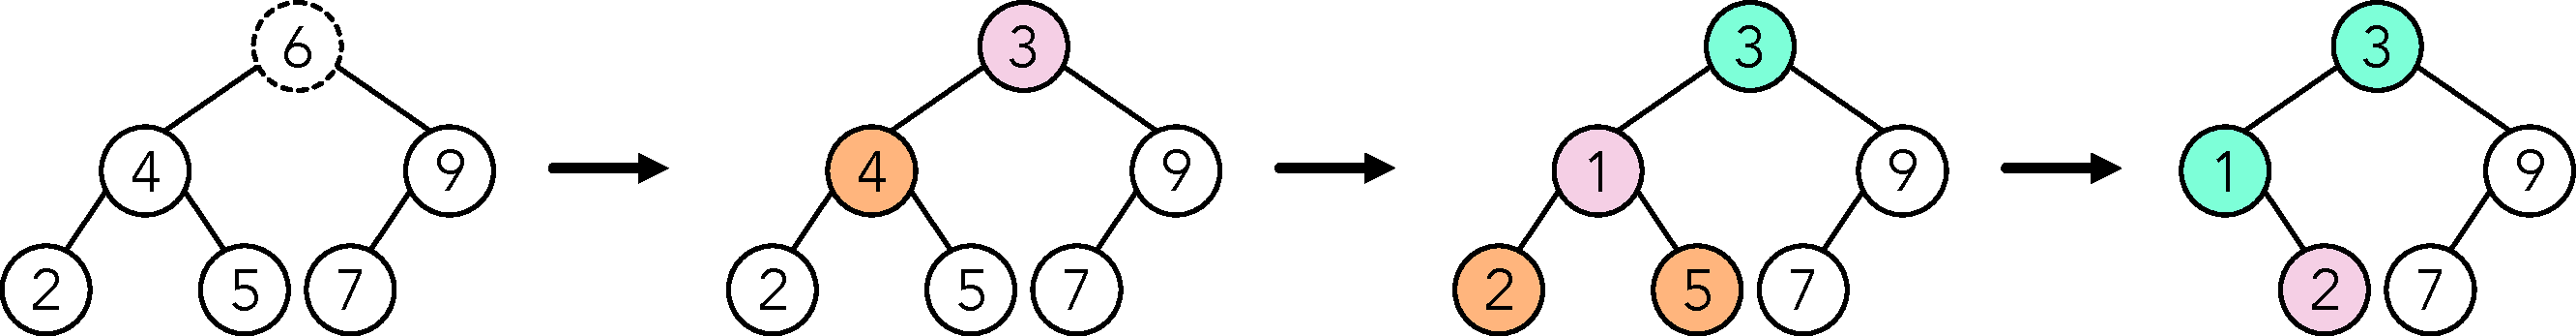
\includegraphics[width=.65\textwidth]{assets/mutate-diagram.pdf}
  \caption{Validity-preserving mutation of a binary search tree, maintaining the
  BST invariant. Mutating the root node from 6 to 3 invalidates the
  4 in the left-hand subtree; the generator 4 with a new random label,
1, then throws away its left subtree (because 1 is the
minimum element of the label range) and relabels 5 to 2.}\label{fig:mutation}
\end{wrapfigure}

Reflective generators can also support
validity-preserving {\em mutation}.
Fuzzing algorithms operate by
mutating ``interesting'' values
so as to explore
the behavior of the program in a space ``around'' those
values. But mutation can be
tricky in scenarios where values are subject to complex validity
constraints, since purely random mutation often produces invalid
values. Reflective
generators can help with this by (1) reflecting on
a particular
value to obtain a sequence of choices, (2) mutate those choices, and (3) run the generator forward with the new
choices, {\em correcting any that
would lead to an invalid value on the fly.} Figure~\ref{fig:mutation}
illustrates how this
algorithm can mutate a binary search tree while maintaining validity,
using no bespoke BST-specific code.

\publicationtarget{Programming Language Design and Implementation (PLDI)}

\SUBSECTION{Usability of reflective generators}{sec:reflectiveusable}{3}{3}{HCI
  Practice}{PhD 2}{PhD 4}{Pierce}
Reflective generators are unavoidably a bit
more complex than standard QuickCheck generators. The current design of the
reflective generator language is a best guess at what users will find most
usable (based on our own experience), but we can do better than guessing!

We will evaluate and redesign the surface syntax of reflective generators with
the help of real users, in a style informed by prior work in the HCI
literature~\cite{ref:ko2015practical}.  We will recruit a small group of users, teach
them to use reflective generators via a short introductory ``README,'' and ask
them to implement a number of PBT generators inspired by the research
literature and real-world examples. We will both observe and interview
the users to identify points of friction and ensure a clear understanding of their
impressions. With this information in hand, we will identify potential changes
to the API and test those changes with a new group of users.  The
ultimate measure of success (again, evaluated through user interviews)
is whether our language for reflective generators is usable by non-expert PBT
practitioners.

\publicationtarget{Human Aspects of Types and Reasoning Assistants (HATRA)}

\SUBSECTION{Generator automation}{sec:genauto}{4}{5}{PL Theory}{PhD 2}{REPL 4}{Pierce}
%
Even with an ergonomic and learnable language for reflective generators, the
less code the user has to write the better. Both of our interview studies
revealed
that thinking about generators slows users down and makes PBT more challenging.
But we should not compromise: any automation should help users obtain {\em high
quality}, {\em reflective} generators for use throughout the testing process.

As a first step, we will adapt existing tools for type-based generator
automation~\cite{mista2019deriving} to work with reflective generators.
In general, type-based
generators are only useful for testing properties with easily satisfiable
preconditions, but this is a good starting point for many developers. Beyond
that, we will consider techniques for {\em interactively}
constructing reflective generators that maintain complex preconditions.

Some users may already have a standard QuickCheck-style generator that
they would like to use
in situations that require a reflective generator. We will assist those
users with tools that automatically synthesize backward annotations
required to make the generator bidirectional. We will experiment with both
conflict-driven program synthesis~\cite{feng_program_2018} and solver-aided
synthesis~\cite{torlak_growing_2013} to see which more successfully generates
annotations for realistic generators.
We plan to collaborate with professor Hila
Peleg at the Technion, who has experience with both PBT and program synthesis. A
letter of collaboration from Prof.{} Peleg appears in the supplemental documents.

Going one step further, we will explore techniques that can synthesize an
entire reflective generator from whole cloth. There are a variety of
attempts to do this for standard generators: Lampropoulos et al. provides
two solutions, one based on on inductive relation specifications of
preconditions~\cite{Lampropoulos&18} and the other based on an
extended language for properties~\cite{beginners-luck}, while Steinh\"ofel et al.
infer a generator from constraints using
Z3~\cite{steinhofel_input_2022,de_moura_z3_2008}.
But none of these
tools fully solves the problem of automated constrained generation in
general, and none of them include the tools necessary to produce reflective
generators.

Pushing forward with generator automation could also extend the reach of PBT
into new domains. Constrained generation is a major difficulty of the
QuickChick ecosystem~\cite{paraskevopoulou_foundational_2015}, and automated
generator solutions could be used to test program
logics~\cite{jung_iris_2018,leino_dafny_2010} to improve usability of PBT in
contexts like proof assistants. More generally, generator automation could make
PBT viable in any situation where properties already exist but preconditions
are hard to satisfy.

\publicationtarget{International Conference on Functional Programming (ICFP)}

\SUBSECTION{Generator benchmark suite}{sec:benchmarks}{1}{2}{Tech
  Transfer}{PhD 2}{PhD 1}{Pierce}
Most papers in the existing PBT literature use small case studies,
showing that certain bugs in certain systems
are caught more quickly with their tool than existing ones. For
theoretically-oriented work, this may be sufficient
to demonstrate the interest of an idea, but such evaluations
are hard to interpret from the perspective of a would-be user.
We can do better.

We have begun work on a robust empirical evaluation framework for
test input generation strategies
including infrastructure
for easily and extensibly running experiments to understand testing
effectiveness.  By ``easily,'' we mean that we will take on the burden of
collecting data and analyzing the results.  When complete, this
evaluation framework will be able to evaluate a given tool based on (1) the
degree to which it is able to achieve high code coverage quickly, and (2) the
speed with which it finds bugs that have been pre-seeded in example programs. By
``extensibly,'' we mean that in addition to the two languages (Haskell and
OCaml/Coq), multiple frameworks (QuickCheck, SmallCheck, QuickChick, etc.), and
numerous workloads that we currently support, we will design the
infrastructure so that users can easily add new
languages, frameworks, and workloads.
Some initial comparisons using this framework will soon be submitted as an experience
report to ICFP 2023, but many crucial features (e.g., coverage measurement) have not yet
been implemented.

Our second contribution will codify a substantial library of case-studies and examples as
{\em benchmarks for PBT}. Similar suites of benchmarks already exist in the
fuzzing literature~\cite{hazimeh_magma_2021}, but those benchmarks are not
organized around the particular challenges that PBT users face. In particular,
few of the benchmarks deal with the kinds of complex preconditions that PBT
tools are built to handle. We want to establish a set of challenging tasks that
can serve as a polestar for future improvements to PBT generators and
bug-finding strategies (including our own!).

Past and proposed work on this topic are joint with Leonidas
Lampropoulos and his group at Maryland.
A letter of collaboration
from Prof.{} Lampropoulos appears in the supplemental documents, and
PI Pierce has a long history
of successful projects with Prof.
Lampropoulos~\cite[etc.]{beginners-luck,DBLP:conf/esop/GoldsteinHLP21,lampropoulos_coverage_2019,Lampropoulos&18,OLDlampropoulos19fuzzchick}.

\publicationtarget{International Conference on Functional Programming (ICFP)}

\SECTION{Specification}{Widening the On-Ramp\pagebudget{2}}{sec:spec}
%
To bring PBT to the people, we need to help developers with envisioning and writing
specifications.
Our the Jane Street study suggested that developers struggle to write
properties about their programs, sometimes due to poorly abstracted code and
other times simply because they fail to imagine what properties they
might want to
test. We propose to address the first of these issues with a
property language that operates over program traces (\sectionref{sec:outpurprop}) and
the second with mixed-initiative interactions where the user and the computer
collaborate to write a property
(\sectionref{sec:interactive}).
%
Further, we will automate one specific high-leverage scenario,
model-based testing (\sectionref{sec:automating}). Finally, we will explore how to
generate automatic explanations of properties, for documentation and
education (\sectionref{sec:understanding}).
%
Success in these tasks will again be measured indirectly, through the
tools described in \sectionref{sec:val} and
\sectionref{sec:diffusion}, and directly in terms of publications.

\SUBSECTION{Properties over program traces}{sec:outpurprop}{2}{3}{PL
  Practice}{PhD 3}{REPL 5}{Pierce}
% With current PBT tools, properties can only be expressed over single modules.
% This causes problems when code is organized with functionality crossing module
% boundaries.
A common pain point for developers in our interview studies was that
their code is not necessarily organized in a way that is conducive to
PBT.  PBT works best on components with clear boundaries and does not
easily apply to programs with
poorly encapsulated global state, or with leaky or complex abstraction
boundaries.

Rather than write properties that are tied to the structure of the program,
we will explore
how to define properties over user-defined
event logs. Consider
the case of a developer we interviewed: P7 was testing
a system, let's call it ``\lstinline{Inner},'' that  was difficult to
test because
its most interesting behavior arose only when interacting with a particular calling
component, ``\lstinline{Outer}''.
\lstinline{Outer} took in simple inputs and used them to construct
much more complex inputs to \lstinline{Inner}. Thus, \lstinline{Inner}
could not be tested with
realistic inputs without the complex apparatus of \lstinline{Outer} to
produce those inputs.  The developer cited this as a circumstance where a
PBT is difficult to apply, because the abstraction boundary between the
components was too fuzzy.

% \TASK{Tools for testing properties over logged values}{2}{2}{Who?}
We plan to develop a tool that allows developers to express properties that reach
into the state of multiple interacting software components. Take again the
example of \lstinline{Inner}. A solution to P7's problem could be to drive the
test through \lstinline{Outer} but write properties about
\lstinline{Inner} by monitoring the internal values that appear while it
runs. For example, suppose
\lstinline{Inner} processes a stream of messages and its internal state
includes a queue of processed items, \lstinline{processed}, and an
\lstinline{overflow} flag. Useful properties might include:

\begin{lstlisting}
prefix_of (processed, next (processed))      (* 1. Processing is monotonic *)
msg.length < 100 ==> never (overflow = true) (* 2. Can handle 100 bytes    *)
eventually (processed.length = msg.length)   (* 3. whole message processed *)
\end{lstlisting}

Is it possible to check such behaviors with built-in assertion statements? We
posit that an assertion-based approach is non-ideal. On the one hand, assertions
would require nontrivial code to save previous values for properties like (1)
above, and likely involves brittle macros or meta-programming to remove such
auxiliary code at release time. Furthermore, it is difficult to imagine using
the assertion approach to checking properties (2) or (3) at all, because it
would require assertions cognizant of the ``end'' of a computation, information
that may not be available to the assertion statement.

Instead, we propose tooling where properties can be defined over logged values.
The first key component of the tool is the invocation of
logging for specific values using lightweight annotations within modules like
\lstinline{Inner}. The second component is a language for writing
properties over the annotations, capable of capturing concepts like \lstinline{next} and
\lstinline{never} from the example properties above. This language will need to
take inspiration from temporal logics, for example linear temporal logic (LTL).

Temporal logics have been used for PBT in prior
work~\cite{oconnor_quickstrom_2022}, but adapting that work to this situation
will require some finesse. For one thing, the prior work assumes a fixed
source of logical events, and thus does not have to support arbitrary predicates
over the kinds of values that may appear in a program trace. For another, LTL is
thought by some to be difficult to use~\cite{greenman_little_2022};
we hope to choose a simplied set of temporal connectives that are
intuitive for users.
%
The end goal of this task is a tool that compiles properties written
in some friendly temporal logic into lower-level properties over log
traces, which are validated by providing random inputs to an outer
system \emph{containing} the component(s) of concern.

\publicationtarget{Object Oriented Programming, Systems, Languages, and Applications (OOPSLA)}

\SUBSECTION{Mixed-initiative property
  specification}{sec:interactive}{4}{4}{HCI Practice}{PhD 3}{PhD 4}{Pierce}
%
Even if a developer believes, in the abstract, that PBT should useful
to them, they may still have trouble writing concrete properties
for real cases that come up in their work. To help build these
intuitions, we will develop
interactive tools to help programmers compose their first
properties in an educational setting.

We envisage a mixed-initiative~\cite{ref:allen1999mixed}
tool, where a student and their code editor work together to arrive at a
meaningful property. Extending prior work on property extraction techniques
\cite[etc.]{ref:ammons2002mining, ref:le2018deep, ref:claessen2010quickspec,
smith_discovering_2017}, the idea is to help students compose properties that
are not just {\em accurate} partial descriptions of correct system behavior, but
that describe {\em important} aspects of behavior. We will build
on a property
extractor that helps students write their first properties by allowing them
to (1) identify areas of code likely to lead to adverse behavior,
(2) provide unit test cases that represent special cases of more general
properties, and (3) select attributes of data types in the source code, or
of input and output relevant data in a debugging REPL.\bcp{Having
  trouble imagining what the previous sentence actually means.} This
will allow a student to more rapidly map from behaviors they can
observe or specify in familiar ways, and see how those behaviors are cast into
the language of their property checker.\bcp{Ditto.}
%
The tool will be deployed in Penn's upper division Haskell
course (CIS 5520) and will therefore be implemented on top of
Haskell's property
generator tool, QuickSpec~\cite{ref:claessen2010quickspec}. \bcp{What
  will QuickSpec be used for, exactly?  I'm not following.}

\publicationtarget{User Interface Software and Technology (UIST)}

\SUBSECTION{Model-based properties for
  modules}{sec:automating}{3}{4}{PL Practice}{PhD 3}{REPL 6}{Pierce}
One finding that surprised us in the Jane Street study is that
it seems to be {very} common for developers to build (or already have) a
{\em model
implementation} of the code they are testing and want to test that
the two implementations behave the same.  This is a
well-documented approach to
  PBT~\cite{hughes_experiences_2016}, but it is not well understood in general,
  nor is it supported as well as it could
be by existing tooling.
%
With this in mind, we plan to build a tool to automate
model-based testing for systems written in languages with strong {\em
  module systems}, like OCaml, Standard ML, etc.~\cite{macqueen_modules_1984}.
We will start in OCaml because our relationship with Jane Street makes it easy
to rapidly get feedback on our findings and tools.

Model-based testing is almost trivial in the case where
the component under test and the model are both pure functions.  But
when the code under test is a {\em
  collection} of functions
organized into a module, things get much more interesting. Testing even a simple
module requires orchestrating multiple calls to the different functions in
its signature. For example, testing the signature \lstinline{StringFns} in
Figure~\ref{fig:sigs} requires wiring together calls the functions in the
signature in a well typed way---e.g., testing \lstinline{drop_n}
requires an integer and a string, each of which must be either generated or
obtained from a call to a different function in the signature (e.g., \lstinline{split}).
We will build on prior
work~\cite{hughes_experiences_2016} to generate well-typed sequences of function
calls that can be used to compare module implementations.

\begin{figure}[t]
  \begin{minipage}{.45\textwidth}
\begin{lstlisting}
module StringFns : sig
  val reverse : string -> string
  val drop_n  : int -> string -> string
  val split   : string -> string * string
\end{lstlisting}
  \end{minipage}
  \qquad\qquad
  \begin{minipage}{.45\textwidth}
\begin{lstlisting}
module Set : sig
  type 'a t     val empty : 'a t
  val mem   : 'a t -> 'a -> bool
  val add   : 'a t -> 'a -> 'a t
\end{lstlisting}
  \end{minipage}
  \vspace{-2mm}
  \caption{Some module interfaces we would like to test
    automatically.}\label{fig:sigs}
\end{figure}

Testing modules gets even hairier when they contain {\em abstract types}, as is
the case with \lstinline{Set}. Now some of the types in the signature cannot be
generated on their own, but must be obtained by
calling other functions in the signature (e.g., \lstinline{create} and \lstinline{add}). The \lstinline{Set} signature is
also {\em polymorphic}, so a concrete instance must be chosen for
the element type \lstinline{'a} before
testing; there is one significant piece of work on this
problem~\cite{hou_favonia_logarithm_2022}, but it is not solved in general.

To address these problems, we will take a foundational approach, breaking down
modules into their constituent features and developing automation
heuristics from first
principles. This will involve identifying a subset of modules, e.g., potentially
those that use generation-unfriendly types like GADTs, where automation is {\em
not} possible; highlighting this subset will provide useful context for future
work that might aim to simplify these cases in other ways (e.g., by putting a
human in the loop). For the modules where our automation does apply, we will
provide a totally automatic solution.

The work in this project will ultimately provide a recipe for automating a
significant swath of module testing situations, massively lowering the
barrier to entry
for PBT in languages with OCaml-like module
systems. It will also
provide a basis that others can
build on in other languages: abstract and polymorphic signatures are features of
many other modularity mechanisms (e.g., Java interfaces, Rust traits, Haskell
type classes, etc.), so solutions we develop for OCaml should
transfer.

\publicationtarget{International Conference on Functional Programming
  (ICFP) and/or Principles of Programming Languages (POPL)}

\SUBSECTION{Automatic explanations for properties}{sec:understanding}{4}{5}{HCI
  Theory}{PhD 3}{REPL 7}{Pierce}
Like any code, properties can
be hard to understand, particularly by programmers who did not write
them. Can we design
tools to help explain them?

We will explore how to design useful in-situ explanations of properties, for example
explanations that could be viewed as just a few lines in
tooltips and inline annotations in the editor and which clarify the meaning
of an opaque property. This involves
several research challenges.

A first challenge is to simply address the right
aspects of complexity; at the minimum, properties can
be confusing because of their use of complex data (e.g., binary search trees,
even logs), structural complexity (as is the cases for properties involving many
predicates), or use of specialized syntax (as happens for advanced properties
incorporating specialized operators in frameworks like QuickSpec). We know all
of these manifest in some properties, but the frequencies are unclear.
We will characterize complexity as it arises
in the properties developers write by conducting a content
analysis~\cite{ref:krippendorff2018content} of code bases using PBT.

A second challenge is understanding how to generate explanations that will help
a programmer understand properties at-a-glance. Several approaches may work well
here.
{\bf Input-Output Examples.} A first approach is to generate
example input-output pairs demonstrating the behavior that a property tests.
This approach is motivated by other recent efforts to generate input-output
examples for instructional
purposes (e.g.,~\cite{ref:gerdes2018understanding,ref:dantoni2015can}).
We will leverage reflective generators and shrinkers to generate
generating understandable inputs with potential complex structure, finding
both positive examples and negative (i.e., failing) examples of program's behavior.
{\bf Plain Language Explanations.} PI Head has prior work developing rule-based textual explainers of
DSLs like CSS selectors and Unix commands~\cite{ref:head2015tutorons}; a similar
approach might work in this context.
The challenge in this research is understanding
patterns of textual explanations that both ``speak the language'' of a reader,
and which can be reliably generated from static analysis of the code.
{\bf Large Language Models.} Large language models have recently
made strides in being able to explain  source code; PI Head is
exploring such technologies for general-purpose programming languages, and this
approach may work well for frameworks like Hypothesis where properties are
written as Python functions.

The above efforts will contribute
a characterization of complexity in property specifications,
techniques for generating readable examples and text descriptions for
properties, and comparisons in
usability studies.

% \publicationtarget{PLATEAU Workshop}
\publicationtarget{IEEE Visual Languages and Human-Centric Computing (VL/HCC)}

\SECTION{Interaction}{PBT at Users' Fingertips
 \pagebudget{3}}{sec:val}
In this section, we
describe a sequence of research efforts to design and evaluate novel modes of
{\em interaction} for PBT. These projects will contribute new
techniques for (1) assessing whether their generators are generating
sufficient and
appropriate inputs (\sectionref{sec:evaluating_distributions}), (2)
altering their generators to achieve better distributions
(\sectionref{sec:tuning}),
and (3) understanding testing-provoked failures involving complex inputs
(\sectionref{sec:failures}).
%
We also describe our plans to design mixed-initiative~\cite{ref:allen1999mixed}
interactions by which a developer could tailor a raw counterexample output by a
PBT tool into the source code for a unit test they would wish to maintain
(\sectionref{sec:counter}).
%
% \bcp{The last, especially,
% may read as ``Just engineering'' to some reviewers.  How do we clarify
% the research content there so that no one can miss it?  E.g., by emphasizing the
% investigate-needs/design/build/evaluate loop? I think addressing this
% point explicitly will help reassure (esp. non-HCI) reviewers.}
% \hg{Is the next paragraph not doing a good enough job here? We could move it
% up maybe?} \amh{Agreed, let me see what I can do.}

Each of these projects will be developed following an
artifact-driven~\cite{ref:wobbrock2016research} HCI research methodology.
In this style of research, contributions come in the form of insights into task 
structure arising from close observational interviews; the creation of novel 
interaction primitives that map closely to these tasks; the refinement of 
technical methods (like those from \sectionref{sec:gen} and 
\sectionref{sec:spec}) to support proof-of-concept implementation; and the 
lessons for interaction and algorithm design that arise from their evaluation 
with human users. Success is evaluated as the interactions' ability to reduce 
testing and debugging time and increase effectiveness.
PI Head has extensive experience with this style of work (see, for 
instance,~\cite{ref:head2015tutorons,ref:suzuki2017tracediff,ref:head2017writing,ref:head2018when,ref:head2018interactive,ref:head2019managing,ref:head2020composing}).

\SUBSECTION{Evaluating data
  distributions}{sec:evaluating_distributions}{2}{3}{HCI
  Practice}{PhD 4}{REPL 8}{Head}
%
Unlike conventional techniques like unit testing, where developers
write concrete test cases,
PBT automatically generates tests by drawing inputs from some
automatically generated distribution. The success of
PBT thus depends on the quality of this distribution---whether
most of its probability mass is on tests that are both sufficiently
''interesting'' and sufficiently diverse.

The challenge is that it is by no means easy for a developer to determine if a 
distribution is a ``good'' distribution. One common strategy is to inspect a 
small number of inputs by hand; though this strategy obviously leaves developers 
without an understanding of the breadth of what is tested by the tests.
Despite advances in HCI in visualizing input data distributions generally,
(e.g., for machine learning model training~\cite{ref:hohman2019gamut} and
~\cite{ref:hohman2020understanding}) and visualizing program sequences of 
program values (e.g.,~\cite{ref:kang2017omnicode}), there remains no fitting 
solution for the PBT case. We aim to remedy that.

More concretely, PBT poses the unique challenge that test inputs are
programmatically generated and
can be of unbounded structural
complexity (e.g., lists, trees, other algebraic data types,
sequences of API calls).
Consider an
example from a participant in our formative study, who wanted to generate
realistic logs of input data, where each log entry included at least a timestamp
and an event type.
% \proposecut{Such values are not trivially plotted in conventional
% visualizations, and it would be prohibitive to review individual examples if the
% logs are sufficiently long.}
Ideally, the developer would be able, by examining the generator's
distribution, to answer
questions like: Are the generated log inputs long enough? and Are the
event sequences
realistic?  This setting requires new kinds of views of data and tight
developer support for easily defining meaningful views of the data.

Our research efforts will focus on developing the interaction primitives 
necessary, and the integration of these primitives, to support rapid 
understanding of generated PBT data. We anticipate making several innovations to 
bring this about. A mockup of these innovations appears in 
Figure~\ref{fig:gen-vis}.

\begin{wrapfigure}{r}{0.58\textwidth}
  \centering
  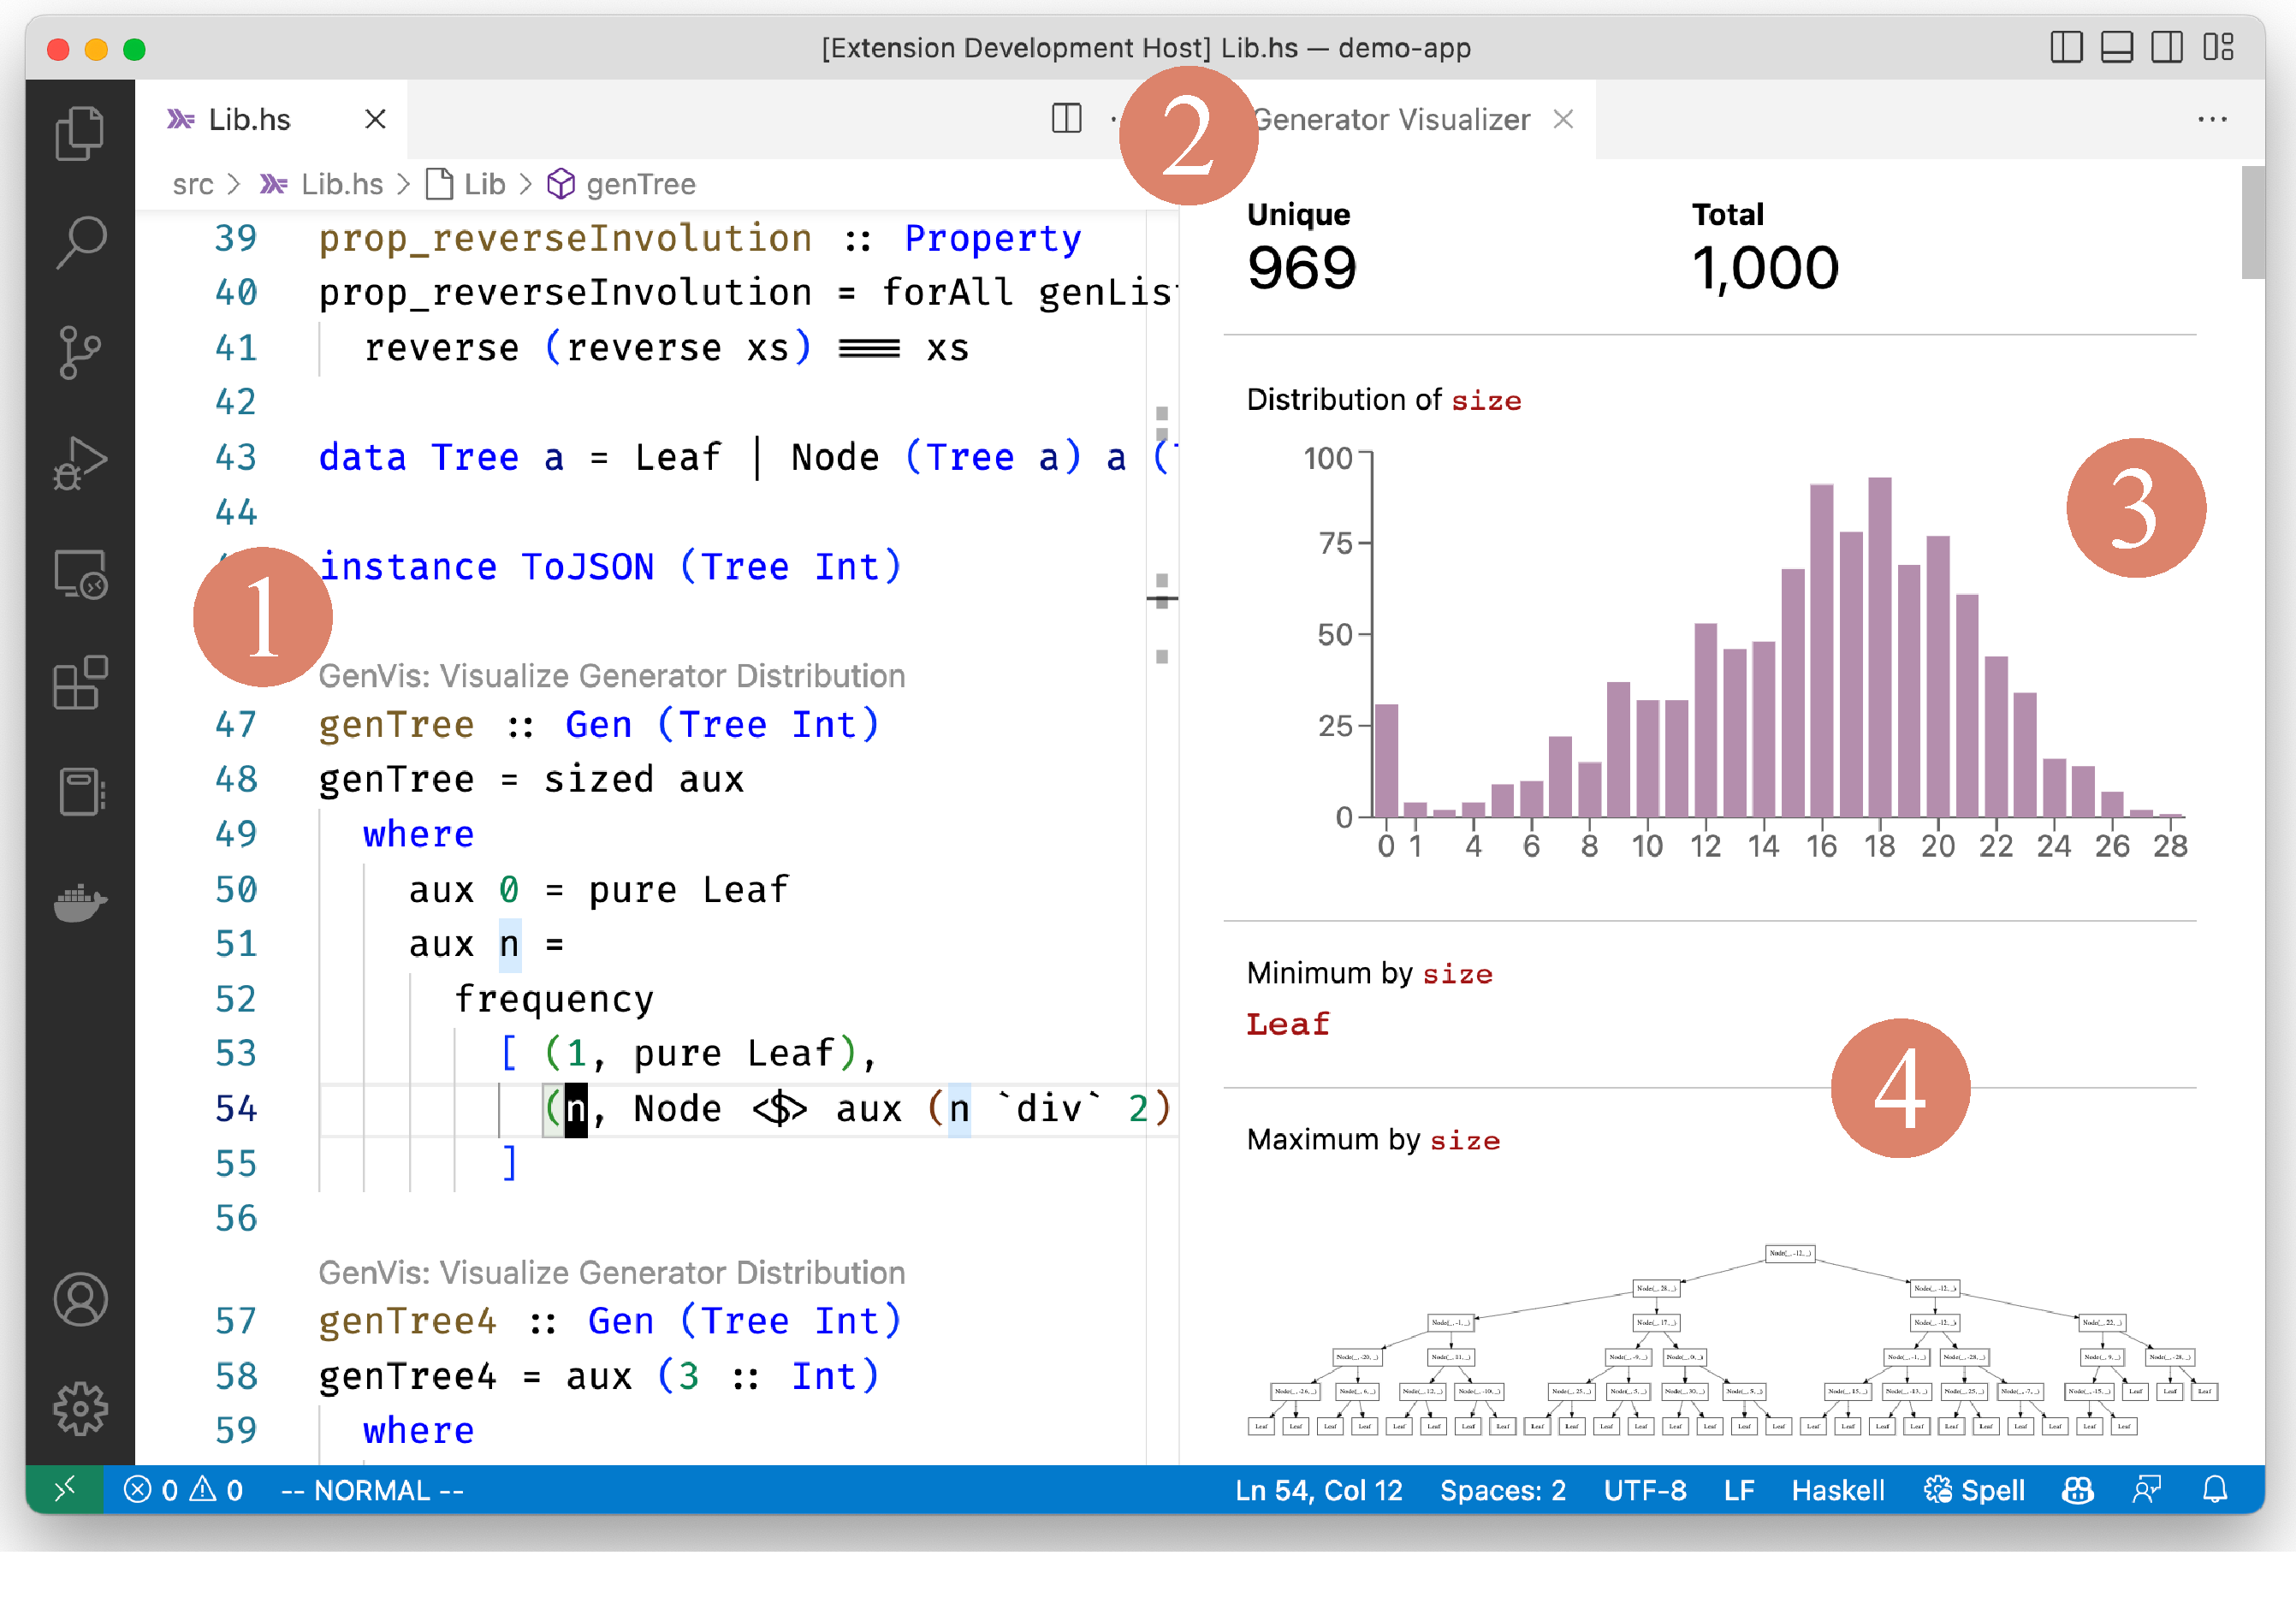
\includegraphics[width=0.58\textwidth]{assets/gen-vis.pdf}
  \caption{A tool for evaluating data distributions, showing
  generator source code (1), summary statistics (2),
  aggregate visualizations (3), and views of input instances
  (4). Iteration would be supported with live adjustment of
  generator code and refinement of filters used in the
  visualizations.}\label{fig:gen-vis}
\end{wrapfigure}

The first research innovation will be the design of live displays of generated 
values. We believe a key requirement will be for these displays to be 
live~\cite{ref:tanimoto1990viva} and real-time. Noting the success of other 
recent live functional programming environments in industry and the lab
(e.g.,~\cite{tool:lighttable,ref:omar2019live}),
our environment will incorporate liveness, sampling values
from the generator and
piping them into data displays. These displays will fill
will first and foremost show aggregate data views, including aggregate
statistics (Figure~\ref{fig:gen-vis}.2) and visualizations of the distribution
of important summary features of the data (Figure~\ref{fig:gen-vis}.3). The 
visualizations will be updated real-time, reflecting values as they are tested 
to allow developers to halt tests upon seeing partial results. Visualizations 
will be
generated according to recommendation rules, as drawn from related work in the 
visualization field~\cite{ref:lee2021lux,wongsuphasawat_voyager_2016,
wongsuphasawat_voyager_2017}. Unique to our setting, the tool will leverage
type-based automation and lightweight user-defined functions to extract features 
to visualize.
For example, consider the
\lstinline{log} type
from above. A developer might be interested in the log's
\lstinline{length}, field accessors like \lstinline{event_type}, \lstinline{id},
and \lstinline{timestamp}, filters like \lstinline{is_empty}, and
aggregators like \lstinline{max_by}. These kinds of features can be
generated automatically for common data types.
% Then the tool will then use
% lightweight type-based program synthesis to compose and combine these functions
% to get features. It may choose to show the \lstinline{length} of a log, but also
% the \lstinline{max_by (fun l -> length l.payload)} (the maximum payload length),
% and even pairs of features like these (which could be viewed as a two
% dimensional feature).

A second innovation will be environmental support for rapid customization with 
user-defined functions.  If
there are features that the developer notices should be extracted but that the
system cannot come up with itself (e.g., \lstinline{ids_unique}), the developer 
can
write them alongside their property specifications;
the interface will automatically load those features into the
display.

A third innovation will be interaction primitives for drilling down into
individual inputs from a list of samples that can be
filtered by selecting marked visualizations (e.g., choose a bar
of length ``10'' to preview individual inputs with that length). Prior HCI tools 
(e.g.,~\cite{ref:hohman2019gamut})
provide this feature generally. What is unique in our domain is to provide 
suitable representations of complex inputs that
will be easy to understand. Some general solutions might be to
pretty-print inputs, provide interactive object browsers like those available
in JetBrains~\cite{tool:jetbrains}, to allow a developer to explore an
object using a built-in REPL, and to produce
DOT~\cite{ellson_graphviz_2002} representations of common kinds of
inputs (i.e., lists, trees) for at-a-glance comprehension of
larger inputs (Figure~\ref{fig:gen-vis}.4). We will try multiple approaches, and 
compare their effectiveness in pilot studies.

A fourth innovation is the synchronization of above views with
live feedback on what code is exercised by the tests. Building on the design 
pattern whereby a tool show which lines of code are currently
executing~\cite{ref:brandt2010rehearse,
  ref:oney2009firecrystal, ref:burg2013record}, our tools will
colorize code to show
how frequently each line is executed while running tests, both in aggregate and 
for individual tests. Altogether, the above activities will be a set of 
interrelated interaction primitives that serve as building blocks for
understanding distributions of complex input data.

\publicationtarget{User Interface Software and Technology (UIST)}

\SUBSECTION{Tuning data distributions}{sec:tuning}{3}{4}{HCI
  Practice}{PhD 4}{REPL 9}{Head}
%
Tuning generator distributions to produce ``interesting''
values more often can be challenging, requiring
significant trial and error. Approaches
like the one in \sectionref{sec:reflective} can help, and in simple cases
heuristics like code coverage are enough~\cite{afl-readme},
but manual tuning
is still sometimes needed.

We will design and evaluate tools to support the direct tuning of
input data distributions
through manipulation of generated inputs and live data distribution
visualizations, building on the foundation outlined in
\sectionref{sec:evaluating_distributions}. Inspired by recent tools in
the PL+HCI literature
for bidirectional manipulation of programs and their
outputs~\cite{ref:hempel2019sketch, ref:kery2020mage,
  ref:omar2012active, ref:omar2021filling},
we will explore reflective generators' potential to support tuning.

One simple way of tuning input data distributions is to
define filters on input data by manipulating aggregate data displays.
For instance, developers could to select a range of values from a bar
chart showing input data features and request that all values in
this range be discarded before testing. This approach is flexible,
but coarse-grained;
it does not influence the implementation of the underlying generator, and
therefore can only go so far in shaping the values that are
generated.  It may also lead to inefficiency, if too many values are
generated from the underlying distribution only to be discarded by the
filter.

A more sophisticated idea is to leverage
reflective generators (\sectionref{sec:reflective}) to change the underlying
generator parameters. Developers will be able to interact with a visualization,
and the the reflective generator will map those interactions
back to choices
in the generator.  The generator code will be displayed
side-by-side with visualizations of the distribution, and the user
will be able to manipulate both sides.
Developers will be able to interact directly with the visualization to
indicate, for example, that they would like to see more inputs like
one that has already
been generated, or that they would like an input similar to a generated input,
but different in a way that they are demonstrating. Together, this tool and the
tool for visualizing generated data distributions will have a synergistic effect
in improving developers' ability to achieve more
realistic, comprehensive data distributions for their testing.

\publicationtarget{International Conference on Functional Programming (ICFP)
and/or User Interface Software and Technology (UIST)}

\SUBSECTION{Interactive shrinking and
  debugging}{sec:failures}{4}{4}{HCI Practice}{PhD 4}{PhD 2}{Head}
%
As in any form of testing, one of the challenges in PBT is understanding why
a given counterexample triggers a bug.  We will design interactive
tools to help.

First, we will design tools that build on
shrinkers~\cite{hughes_quickcheck_2007,arts_shrinking_2014} to help developers
understand counterexamples. Automatic shrinking, even when done via reflective
shrinkers as we discuss in \sectionref{sec:reflective}, can be opaque, and
shrinkers can get stuck at local minima that are far from the global minimum.
But developers can often see shrinking options that the shrinker does not know to consider.
Drawing inspiration from approaches in recent HCI literature that support
interactive code reduction through iterative, incremental
experimentation~\cite{ref:lim2018ply,ref:head2018interactive,ref:holmes2012systematizing,ref:hibschman2016telescope},
we will experiment with aids for rapid, incremental, interactive
shrinking of complex
inputs into simpler ones. The key feature we will develop is the ability to
shrink inputs semi-automatically by manipulating them in an interactive
object viewer, similar to the viewers available in contemporary
debuggers like in the JetBrains IDE~\cite{tool:jetbrains}.

An interactive shrinker can display the valid ways in which an input
can be pruned,
relying on reflective generators to provide the insights into which parts of the
structure correspond to changes that do not break program preconditions.
Alternatively, the developer might change
the input entirely, for example, noticing some change of inter-dependent parts
of the structure that shrinking missed.  As a developer manipulates the input,
automatic shrinking will continuously be re-tried, reducing the input further
and giving feedback as to whether it still causes a test to fail or not.
Developers will ultimately be able to reduce complex counterexamples into
simpler ones that are easier to reason about when looking for bugs.

% Notes from Andrew
% Why hypothesis 'explain' won't work:
% * The existing strategy is not quite right---sometimes the challenge is not
% due to lines that are always run on failure, but rather the absence of
% important lines. Still, these challenges can be predicted by a different
% number of runs through the same control statements. Furthermore, someone may
% wish to not just know the difference in which lines were run, but to step
% through execution of them side by side.
% * A tool like TraceDiff could be used, if integrated into a conventional
% editor. That said, we expect it would not fit in without novel interaction
% solutions, particularly because...
% * We don't know the correct program, so we can't compare the trace to the
% correct program. Instead, all we have is the traces of other correct
% executions. It is likely, then, that we have to...
% * Show multiple inputs stepping through the same code at once.
% * Highlight control divergences (through simple highlighting). Dump people in
% the location of the first control divergence and visualize it.
% * (Maybe) Permit the ability to step backward
% * Convey this through subtle highlighting, perhaps weighted by the number of
% inputs that travel particular paths to reveal scent, and highlight paths that
% are *not* executed. Refine these design choices on the basis of bugs that we
% learn about by mining repositories.

In addition to developing novel interaction techniques for simplifying inputs,
we will also develop systems for helping developers locate code that, if
changed, would resolve the failure. Rather than explicitly encoding
relationships between generated test inputs\bcp{inputs generated by the
  generator?  outputs generated from those inputs by the SUT?}
\hg{I don't know Ko's work enough to grok this. @Andrew?}
and their dependencies on
code~\cite{ref:ko2009finding}, we will instead help the developer
understand where the execution path for a given counterexample diverges from
similar, successful inputs.
Leveraging
reflective generators, we will generate inputs in a space ``around'' a
counterexample and identify which ones no longer cause a failure.  Then, we will
execute the program up to the point where the traces begin to
diverge and drop the programmer into a debugging environment where
they can query the state of the program and step through the remainder of the
execution. PI Head has prior work designing debugging tools that help
programmers understand trace divergences in an educational
setting~\cite{ref:suzuki2017tracediff}.

\publicationtarget{User Interface Software and Technology (UIST)}

\SUBSECTION{Counterexamples as regression
  tests}{sec:counter}{5}{5}{HCI/PL Practice}{PhD 4}{REPL 10}{Head}
%
% After testing has revealed a counterexample to one of their properties
% with their tests, the developer may wish to turn that failure into a
% regression test, to ensure that later
% changes to the code will not reintroduce the same failure.
One pain
point reported
by informants in our Jane Street interviews was that it requires
considerable work to
transform a failure detected by their PBT tools into a
regression test, even though much of this work
feels mechanical.

In reality, the work is \emph{mostly}, but not entirely, mechanical.
Creating good regression tests will require judicious incorporation of
the developer's input at key decision points, particularly for
specifying acceptance criteria\bcp{what's that?}. For instance, consider a property that checks
that a list insertion function never produces an empty list. In the event of a
failure, a developer may want to produce a regression test checking the
exactness of the result on the failed input (e.g., checking that the insertion
produced a particular concrete list) rather than simply checking that the output
list is non-empty.\bcp{I don't get this.  Is the regression test
  supposed to test the {\em in}correct behavior, or the correct
  behavior after the bug is fixed?  Why would we want the former?} \amh{The
  correct behavior, though the property may underspecify the intended output
  versus what the developer would like to have in the test.}
Writing a regression test may involve multiple such
choices, including whether to test for exact output, whether to test
intermediate results, and how to initialize inputs.\bcp{Readers may
  have trouble visualizing why we'd need each of these.}

We will explore interactive tools to assist developers in creating
regression tests from failed tests. The idea is to first develop
technology for generating sufficiently readable code for regression
tests\bcp{I don't have a clear picture of what this would involve.
  Isn't a regression test just ``You poke the system like this and it
responds like that''?  Where are the readability challenges?}\amh{I think it
is more stylistic questions than any. An automated test case generator might
produce a test that is technically correct, but ugly. For instance, multiple
function calls are chained in the same line, rather than split onto multple
lines. Or test success is evaluated by comparing to a really complex output,
rather than comparing one particular attribute on that output that you really
care about. These are types of stylistic choices that may be difficult to encode
in an automated test case generator / styler, but something that would be pretty
easy for a person to identify as improvements to the test case.} (using
approaches such as Daka et al.'s~\cite{ref:daka2015modeling}), and then provide
in-situ editing assistance along the lines of contemporary interactive
refactoring tools from the HCI
literature~\cite{ref:head2018interactive,ref:barik2016quick,ref:murphyhill2008refactoring,ref:lee2013draganddrop}.
For this specialized task of transforming properties into regression tests,
our tool will provide a few key features:
keeping track of the failed input,
generating starter test code, substituting in correct expected values of the
output by executing corrected code, and supporting developers in rapidly
performing likely edits to regression tests.%
\bcp{Again, I'm worried that (especially for non-HCI reviewers) this
  will read like ``Oh, they want to build a little tool,'' rather
  than, ``This is a research topic that one could write a whole paper
  about.''}\amh{I need to think about this.}
We also hope the results of this work
can inform the
design of other approaches to counterexample extraction, including one that is
proposed for the Hypothesis in Python.\bcp{Going into more detail
about this bit might help!}\amh{I'm not sure about this one; I think this is
based on Harry's communication with Zac. One of us should either turn Zac's
feedback into something concrete here, or otherwise we should leave it out.}

\publicationtarget{Foundations of Software Engineering (FSE)}

\SECTION{Diffusion}{Advancing Open-Source Tools}{sec:diffusion}
The activities described in the previous sections are focused on
fundamental research to advance understanding of PBT and explore new
approaches both foundations and tool design.  But research alone is
not enough to reach the broad impact we seek. Accordingly, our agenda
includes plans for increasing the {\em diffusion} of PBT through both
educational materials and well engineered tools
embodying our findings.

We begin with activities for ensuring that our foundational
advances have an impact on real users, with the help of a research
engineer (\sectionref{sec:engineersupport}). A major part of this
effort will be
building and maintaining \tyche, an integrated development environment for PBT
(\sectionref{sec:ide}). Next, we discuss plans for helping
support open-source frameworks for PBT (\sectionref{sec:nurturing}).
Finally, our
education-focused activities include a catalog of high-leverage PBT
use-cases (\sectionref{sec:whento}) and undergraduate- and
masters-level courseware for PBT
(\sectionref{sec:1210}).

In addition to code and educational materials, the projects in this section will
also result in a number of engineering-focused talks. We will bring these talks
to industry conference like ``Yow! Lambda Jam,'' ``Strangeloop,'' and
``Lambda World.''

\SUBSECTION{Beyond research software}{sec:engineersupport}{3}{5}{Tech
Transfer}{Engineer}{}{Pierce}
%
The research projects described above have the potential to
dramatically improve the power and usability of PBT, but only
if their products are attractive to real users. There is an unfortunate tendency for
research software to remain just that---missing critical
documentation that new users need to get started and lacking a clear
maintenance schedule that would give software companies the confidence
to adopt.
To avoid this fate for our projects, the PhD students will work closely with our
research engineer. The code for those projects will be designed with learnability and
maintainability in mind, and upon
completion it will be handed off to the
engineer to grow and maintain.

Concretely, we expect the research engineer to be most involved in the following
projects. {\em PBT interaction models}~(\sectionref{sec:understanding}): Helping PhD
  1 to build and maintain a minimal PBT framework for use in comparison studies
  and as a model for future PBT frameworks.
  {\em Theory of reflective generators}~(\sectionref{sec:reflective}):
  Implementing and maintaining versions of reflective generators in a number of
  languages and PBT ecosystems, with the help of PhD 2.
  {\em Mixed-initiative property
  specification}~(\sectionref{sec:interactive}) and {\em Counterexamples as
  regression tests}~(\sectionref{sec:counter}):
  Assisting PhD
  3 with maintenance of tools for easier property specification.
%
Most importantly, the research engineer will help to build and maintain
\tyche{}, the IDE for PBT designed as part of PhD 4's dissertation. We
describe this effort in more detail in the next section.

\SUBSECTION{Tyche: An IDE for PBT}{sec:ide}{2}{5}{Tech
  Transfer}{Engineer}{PhD 4}{Pierce}
The projects in \sectionref{sec:val} will explore a wealth of new modes of interaction
for PBT. Their potential impact will be significantly magnified if they are
integrated together in a
place that is easily accessible to would-be users. This is the inspiration for
\tyche{}, an integrated development environment (IDE) extension for PBT.

\tyche{} will include all of the functionality designed in \sectionref{sec:val},
including tools that facilitate guided PBT
workflows, help developers tune and
improve generators, and assist in the property-authoring
and debugging processes---all integrated into Visual Studio Code. A 2022 survey~\cite{noauthor_stack_nodate}
showed that VSCode is the most widely-used IDE, and it has support for every
language that currently has significant PBT support.
While \tyche{} is intended to be language-agnostic where possible, the Hypothesis
developers have even recommended that we try to include a fork of
\tyche{} into the main Python language extension for VSCode.

The research engineer will assist in the integration process, ensuring that the
extension is more than the sum of its parts. Indeed, we plan for \tyche{} to
live on as a home for further innovation: future tools that we or others in the
community see as important improvements to PBT workflow will also be included
over time.  With a strong theoretical grounding and consistent engineering
support, \tyche{} will provide an efficient pipeline for bringing research on
PBT interaction models to developers craving better tools.

We will popularize \tyche{} through talks at developer
conferences and by
disseminating information via our contacts in industry and the open source
community.
%
% We will list the IDE on the Visual Studio Code extension marketplace,
% with a goal of reaching 60,000 downloads by the end of the project.
We aim for \tyche{} to reach 60,000 downloads by the end of the
project. At
the time of writing, this would put \tyche{} in the top 10 extensions
tagged ``Testing'' in the Visual Studio Code extension marketplace
that are not either full language servers or Large
Language Model interfaces~\cite{noauthor_testing_nodate}.

% We aim for \tyche{} to reach 60,000 downloads by the end of the
% project, driven, in part, by our connections in the developer tool community.

\SUBSECTION{Nurturing the PBT ecosystem}{sec:nurturing}{1}{5}{Tech
Transfer}{Engineer}{PhD 1}{Pierce}
The existing ecosystem of open-source PBT tooling is broad and varied. Some
projects are vibrant, while others, including some with
great ideas and implementations, do not have the developer bandwidth to address
user needs. Additionally, existing frameworks have not been designed with
the benefit of the insights and tools that we will build in this
project, leaving (we believe) large opportunities for improvement.
Thus, we will allocate a significant part of the engineer's time to
supporting and improving open-source PBT frameworks.
%
To make best use of limited resources, we will choose three existing PBT
frameworks as targets and use the findings and software products from
our research to boost their usability and adoption.

We will start
with Python's Hypothesis framework, since it is well-established and yet has
significant room for growth.  We are in contact with Zac Hatfield-Dodds, the
main maintainer; a letter of collaboration from Mr.{}
Hatfield-Dodds appears in the supplemental documents. The Hypothesis team is
especially excited about integrating ideas like reflective generators
(\sectionref{sec:reflective}) and interaction modes like distribution
visualization (\sectionref{fig:gen-vis}) into Python's VCSode environment.
The success of this collaboration will be measured by the Hypothesis team's
willingness to include our tools in future releases and promote them to the
community.

Besides Hypothesis, we will seek out two more projects to work with. These
will be chosen based on potential impact: we will prioritize great
projects in popular programming languages that have significant room
for growth. Candidates include
Scala's ScalaCheck,
OCaml's Crowbar, which is not actively maintained but has great ideas and
some attractive low-hanging fruit~\cite{noauthor_shrinking_nodate}, and projects like
\lstinline{jqwik} in Java or \lstinline{proptest} in Rust, which are
embedded in massive language
communities that could benefit from better tools for PBT. Whichever
projects we choose, we will either take them over (if
unmaintained) or work closely with their
developers to ensure that our input is well received by the community.

\SUBSECTION{``When to Specify
  It!''}{sec:whento}{1}{1}{Education}{Faculty}{Everyone else}{}
%
Besides engineering efforts, we plan to disseminate PBT via
educational materials.
% Our first pilot study with users of PBT suggested that developers struggle to
% come up with specifications that are worth
% testing~\cite{goldstein_problems_2022},
% but
% our follow-up
Our interviews at Jane Street suggest that the developers there
% rarely have the same problem. It seems that the Jane Street developers had
have a tacit
understanding of several ``no-brainer'' situations where PBT is an obvious
choice, situations where properties are easy to find and PBT provides
more thorough testing than other techniques---indeed, many developers
seem to limit their use of PBT to such situations.
While experienced PBT users do also apply it in
high-cost / high-benefit situations, it appears that
focusing educational efforts on easy cases may be the best way to
drive adoption.

We will produce resources to help developers understand
high-leverage situations for PBT. We will begin with an effort
tailored to the academic community: a survey paper with the
aspirational title ``When to Specify It!'' in homage to John Hughes's
widely-viewed tutorial ``How to Specify It!''. This survey will
document a  range of high-leverage scenarios identified in our formative
research, including cases like
\begin{enumerate*}[label=(\arabic{enumi})]
\item ``these two functions (e.g., a parser and a printer) should round-trip,''
\item ``this data structure (e.g. a set, map, etc.) should obey algebraic laws,''
\item ``this stateful module should uphold an invariant,''
\item ``these two programs should behave the same'' (e.g., because one
is an optimized version of the other),
and
\item ``this program should not crash.''
\end{enumerate*}
This list will be expanded based on follow-up surveys with broader
communities of developers~(\sectionref{sec:survey}), a comprehensive
review of case studies that appear in
the academic literature, and an examination of open source projects across a
variety of different software ecosystems using PBT (e.g.,
QuickCheck/Haskell, Hypothesis/Python, Quickcheck/OCaml).

We will distill these findings
into media directly tailored for developers. First, we will write
approachable developer documentation in partnership with our industry
collaborators, to be read among the first resources of any developer
documentation on PBT tools. We will work with our industry collaborators to
disseminate this documentation and incorporate it into blogs and tool
manuals. Finally we will package the findings as a talk for one or more
professional conferences.

\SUBSECTION{Curricula for PBT}{sec:1210}{1}{5}{Education}{Faculty}{Engineer}{}
%
Education can act as a force multiplier to drive adoption of new
technologies in industry.
We will develop materials for
integrating PBT into early undergraduate courses---initially targeting
introductory data structures
courses---as well as higher-level courses for masters students. As noted in \sectionref{sec:whento}, testing well-defined data
abstractions is one of the high-leverage scenarios for using PBT, making data
structures a powerful anchor for demonstrating the power of PBT.
%
Building on
recent PBT teaching in data structures
courses~\cite{wrenn2021using,nelson2021automated}, we will integrate PBT into
Penn's CIS 1210 course on data structures (which PI Pierce regularly teaches).
%
We
will evolve the CIS 1200 curriculum to emphasize themes in PBT from our
formative research---good circumstances for
using PBT, methods for writing useful generators, properties as
documentation, and scenarios where PBT is suitable
(see~\sectionref{sec:whento}).
%
We will also include PBT in Penn's CIS 5730, a masters-level software engineering
course.
%
We will evaluate the impact of these new
instructional approaches on students' ability to leverage PBT in final projects,
disseminating our findings in publications at computer science
education venues.
%
The instructional materials we develop will be made available for instructors at
other institutions to use in their own courses.

\publicationtarget{Koli Calling International Conference on Computing Education Research}

\immediate\closeout\workplanfile
% \SIMPLESECTION{Plan of Work\pagebudget{.7}}{sec:plan-of-work}

% \bcp{I've moved the text that was here to a separate supplemental
%   document, but we'll probably want to say something short in the main
%   project description (either here or, better, toward the top) about
%   synergy and coordination, with a pointer to that document.}

% \begin{figure}[ht]
%   \centering
%   \vspace*{-1in}
%   \hspace*{-.4in}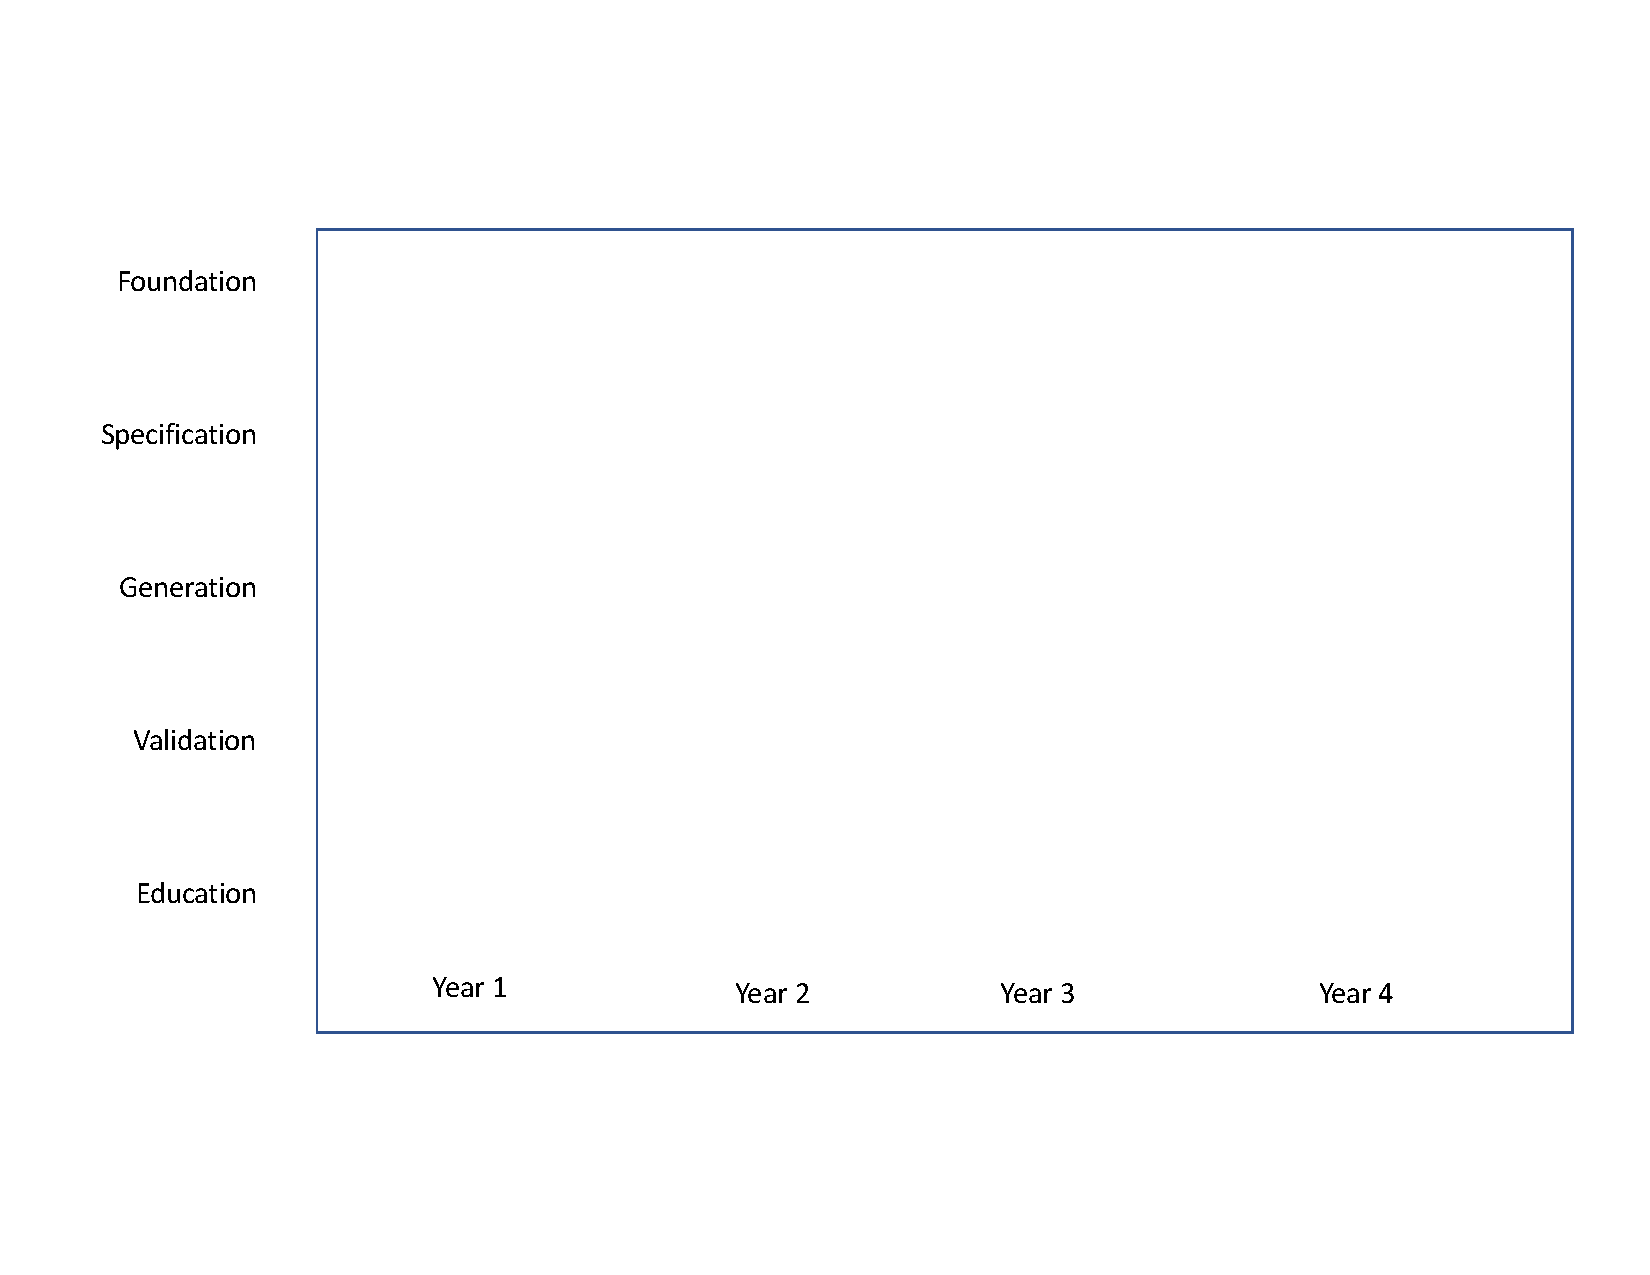
\includegraphics[width=1.1\textwidth]{assets/workplan.pdf}
%   \vspace*{-1.3in}
%   \caption{Plan of work.}\label{fig:workplan}
% \end{figure}

% \vspace*{-.4in}


\SIMPLESECTION{Broader Impacts%
 \pagebudget{.5}}{sec:broader-impacts}

Broad impact is central to our research agenda, and many of the specific
tasks we have described---particularly those grouped under Diffusion
(\sectionref{sec:diffusion})---aim for broad impacts.  Here we
recapitulate those aims and sketch our plans for mentoring, diversity,
and broadening participation in computing.

\smallskip
\noindent{\bf Impact on industry.} The main broad impact from the
proposed work will be a significant increase in the use of PBT across
the software industry within the time frame of the grant, driven
by more powerful and usable tools. Specifically, the research engineer will work to
bridge the gap between the foundational insights and prototype tools
coming from the four PhD students and the needs and priorities of
industrial developers.
Specific activities led or amplified by the research engineer are discussed in
\sectionref{sec:engineersupport} and \sectionref{sec:nurturing}.

\smallskip
\noindent{\bf Educational Impact.}
%
A second, supporting arena for broad impact will be the
development of educational materials for both students and
professional developers. Educational activities will be
coordinated with the rest of the work, and they are integral to the
project's overall goal of making PBT a standard testing methodology.
Specific pedagogical
threads within the project are described in \sectionref{sec:whento} and \sectionref{sec:1210}, but the
tasks in \sectionref{sec:foundation}, \sectionref{sec:reflectiveusable},
\sectionref{sec:interactive}, \sectionref{sec:understanding}, and
\sectionref{sec:evaluating_distributions} will also influence education. The
work in \sectionref{sec:1210} in will generate course materials that we will
share publicly; we will also report our experiences in a paper for a
CS-ed-focused conference or journal.

An ancillary educational goal is to
publicize and communicate the benefits of PBT to the broader computer science
{\em research} community. As part of these efforts, we will write an article on PBT
for the Communications of the Association for Computing Machinery
(CACM).

\smallskip
\noindent{\bf Mentoring and Diversity.}
%
The majority of the requested funding will support formative research
experiences and mentoring for graduate students. We
also plan to work with 10 undergraduate students via an
REU program (more in the next paragraph) along with other
undergraduate and masters
students working for credit;
they, too will benefit from the research experience. Each graduate
student will have leadership responsibility for multiple facets of the
project, including co-supervising interested undergraduate and masters
researchers.

The PIs will recruit students for this project with a mind towards making
the research area reflective of diversity in the US and Pennsylvania.
The PIs have already made inroads broadening participation of women in their
groups (1/3 of Pierce's direct Ph.D. mentees and 2/3 of PI
Head's are women). That said, a particular area of focus going forward
will be increasing representation of
other underrepresented groups, including Black and Latinx
students. Pierce (along with Penn colleagues Zdancewic and Weirich)
was recently informed that he will receive funding for an
NSF REU program that will involve 24 undergraduates (either per
year for three+ years), selected specifically with an eye to diversity;
for the present project, we are requesting funds to add two more per
year specifically to work on PBT topics, many of which are well suited
to undergraduate interns. See the Broadening Participation in Computing supplementary
document for more details.

\smallskip
\noindent{\bf Benefits to Society.}
%
The project's goals will also be advanced by open-source distribution of tools
built during the project. Key systems will be engineered and documented to a standard
that makes them immediately useful to engineers and students; the projects around
improved generation and shrinking, PBT over logs, and evaluating data
distributions will be particular targets for widespread
dissemination. The remaining projects will be published under a permissive
open source license to serve as models for similar tools in other
programming languages and environments.

This project also presents excellent opportunities for strengthening
collaborations between university researchers and industrial advocates of PBT.  Our
ongoing user study at Jane Street has been carried out with the
enthusiastic support of their developers and management, and we hope
to continue using Jane Street as a testbed for prototypes of our
tools.  We are also in active discussions with the
developers of Hypothesis, who are keenly
interested in the results of this proposal.
We plan to establish connections with the
developers and user communities of popular PBT tools in languages like
Java, Rust, and Scala.

Longer term, better testing means better software.  As software
systems have grown to the gigantic scale seen today, good testing
methodologies and tools (unit testing tools, test-first design
methods, etc.) have come to play an ever more crucial role.  Adding a
powerful new testing tool to programmers' toolbelts will further streamline
this aspect of the development process, leading to software of every
sort that is more robust, more reliable, and less expensive.


% \proposecut{See the Collaboration Plan for
% more.}

% The Project Description must contain, as a separate section within the narrative, a section labeled ``Broader
% Impacts of the Proposed Work". This section should provide a discussion of the broader impacts of the proposed
% activities. Broader impacts may be accomplished through the research itself, through the activities that are
% directly related to specific research projects, or through activities that are supported by, but are complementary to
% the project. NSF values the advancement of scientific knowledge and activities that contribute to the
% achievement of societally relevant outcomes. Such outcomes include, but are not limited to: full
% participation of women, persons with disabilities, and underrepresented minorities in science, technology, engineering, and
% mathematics (STEM); improved STEM education and educator development at any level; increased public
% scientific literacy and public engagement with science and technology; improved well-being of individuals in
% society; development of a diverse,globally competitive STEM workforce; increased partnerships between
% academia, industry, and others; improved national security; increased economic competitiveness of the United
% States; and enhanced infrastructure for research and education.

\SIMPLESECTION{Results from Prior NSF Support\pagebudget{.5}}{sec:prior}

% If any PI or co-PI identified on the project has received NSF funding (including any current
% funding) in the past five years, in formation on the award(s) is required,
% irrespective of whether the support was directly related to the proposal or not.
% In cases where the PI or co-PI has received more than one award (excluding amendments),
% they need only report on the one award most closely related to the proposal. Funding includes not just salary
% support, but any funding awarded by NSF. The following information must be provided:\\

\emph{\underline{PI Pierce}}: (NSF 1955565) ``Collaborative Research:
SHF: Medium: Bringing Python Up to Speed'' (\$437,999,
7/2020--6/2023), with co-PIs Michael Hicks (Maryland) and Emery Berger
(Amherst).
The project aimed to dramatically increase the performance and
correctness of applications written in Python by developing novel
techniques for performance analysis, optimization, run-time systems,
property-based random testing, concolic execution, and program
synthesis. It developed both
novel performance analysis tools and optimizations and novel automatic
testing frameworks. These were largely tailored to and implemented for
Python, but applicable in other, similar languages.
%
{\bf Intellectual Merit.} The project involved work on both
performance measurement (mostly at Amherst and Maryland) and PBT (mostly at Penn
and Maryland).  Specific threads of work involving Penn included
building an early
version~\cite{Frohlich2022} of the Reflective Generators described in
\sectionref{sec:reflective}, carrying out the pilot study of PBT in Python
mentioned in the motivation section
above~\cite{goldstein_problems_2022}, and building on the idea of
freer monads from functional programming to develop ``free
generators,'' which unify parsing and
generation~\cite{goldstein2022parsing}, presented a principled
automatic testing framework for application-layer
protocols~\cite{Li2021:MBToNA}, and developed and released a freely
available mutation testing framework for Python, called {\tt
  pytest-mutagen}~\cite{pytestmutagen}, and applied ideas from
combinatorial testing, a widely studied testing methodology, to modify
the distributions of random test-case generators so as to find bugs
with fewer tests~\cite{DBLP:conf/esop/GoldsteinHLP21}.
%
{\bf Broader Impacts.} Project results and open-source software
products are being used to increase the
performance and correctness of Python applications.
Educational impact has included training both graduate and
undergraduate students, including a female PhD student at Penn, Jessica
Shi.
%
{\bf Publications (involving Penn):} \cite{Frohlich2022,DBLP:conf/esop/GoldsteinHLP21,
  goldstein2022parsing, goldstein_problems_2022, Li2021:MBToNA}.
{\bf Research Products (involving Penn)} \cite{pytestmutagen}.

\smallskip

\noindent\emph{\underline{PI Head}} has not previously received NSF support.

% \SUBSECTION{Proposed Study}{}{}
% The Project Description should provide a clear statement of the work to be undertaken and must include:
% objectives for the period of the proposed work and expected significance; relation to longer-term goals of the PI's
% project; and relation to the present state of knowledge in the field, to work in progress by the PI under other
% support and to work in progress elsewhere.
%
% The Project Description should outline the general plan of work, including the broad design of activities to be
% undertaken, and, where appropriate, provide a clear description of experimental methods and procedures.
% Proposers should address what they want to do, why they want to do it, how they plan to do it, how they will
% know if they succeed, and what benefits could accrue if the project is successful. The project activities may be
% based on previously established and/or innovative methods and approaches, but in either case must be well
% justified. These issues apply to both the technical aspects of the proposal and the way in which the project may
% make broader contributions.
